%%%%%%%%%%%%%%%%%%%%%%%%%%%%%%%%%%%%%%%%%%%%%%%%%%%%%%%%%%%%%%%%%%%%%%%%%%%%%%%

\documentclass[12pt,twocolumn,tighten]{aastex63}
%\documentclass[12pt,twocolumn,tighten,trackchanges]{aastex63}
\usepackage{amsmath,amstext,amssymb}
\usepackage[T1]{fontenc}
\usepackage{apjfonts}
\usepackage[figure,figure*]{hypcap}
\usepackage{graphics,graphicx}
\usepackage{hyperref}
\usepackage{natbib}
\usepackage[caption=false]{subfig} % for subfloat
\usepackage{enumitem} % for specific spacing of enumerate
\usepackage{epigraph}

\renewcommand*{\sectionautorefname}{Section} %for \autoref
\renewcommand*{\subsectionautorefname}{Section} %for \autoref

\newcommand{\cn}{NGC\,2516} % cluster name

% gaia target sample numbers
\newcommand{\nkinematic}{3{,}298} % "fullfaint" kinematic sample, core+halo (CG18+KC19+M21). from any call of earhat.helpers._get_fullfaint_dataframes
\newcommand{\nnbhd}{13{,}843} % make_compstar_NGC_2516_sourcelist.py
\newcommand{\ncore}{1{,}106}  % "fullfaint" kinematic sample, CG18. from any call of earhat.helpers._get_fullfaint_dataframes
\newcommand{\nhalo}{2{,}192} % "fullfaint" kinematic sample, KC19+M21. from any call of earhat.helpers._get_fullfaint_dataframes

% from drivers.cluster_rotation.get_auto_rotation_periods.py;  checked with plot_target_vs_actual_list_sanity_checks.py
\newcommand{\ncdips}{2{,}205}
\newcommand{\nkinematicrpltsixteen}{2{,}270}
\newcommand{\nkinematicCGandKC}{2{,}236}

% cdips results numbers
\newcommand{\numcdipslcs}{671{,}901} % drivers.yield_calculation.count_cdips_lcs.py; 2021.01.13
\newcommand{\numsouthernuniqlcs}{483{,}407} % drivers.yield_calculation.count_cdips_lcs.py; 2021.01.13

\newcommand{\ncalibration}{9{,}619{,}784} % /nfs/phtess2/ar0/TESS/PROJ/lbouma/CDIPS_LCS/counts/check_sum, 2021.02.02
\newcommand{\nnbhdcaliblc}{9{,}790} % get_auto_rotation_periods.py
\newcommand{\nnbhdcalibstar}{1{,}987} % get_auto_rotation_periods.py

\newcommand{\nautorotdenominator}{1{,}641} % plot_autorotation.py, w/ runid=NGC_2516. For nequal<=0, nclose<=1, LSP>0.08. See /doc/20210205_nequal_and_Prot_vs_color_cleanup.txt
\newcommand{\nautorotnumerator}{987} % plot_autorotation.py, For nequal<=0, nclose<=1, LSP>0.08. See /doc/20210205_nequal_and_Prot_vs_color_cleanup.txt
\newcommand{\nautorotnumeratormatching}{507} % plot_autorotation.py, LSP=SPDM period
\newcommand{\ncompstardenominator}{820} % plot_autorotation.py, w/ runid=compstar_NGC_2516. For nequal<=0, nclose<=1, LSP>0.08. 
\newcommand{\ncompstarnumerator}{365} % plot_autorotation.py
\newcommand{\ncompfrac}{44.5\%} % plot_autorotation.py
\newcommand{\nautovscompstardenominator}{705} % plot_autorotation.py, w/ runid=compstar_NGC_2516. For nequal<=0, nclose<=1, LSP>0.08. 
\newcommand{\nautovscompstarnumerator}{374} % plot_autorotation.py
\newcommand{\nautofrac}{53.1\%} % plot_autorotation.py

\newcommand{\kms}{\,km\,s$^{-1}$}
\newcommand{\ms}{\,m\,s$^{-1}$}
\newcommand{\bpmrp}{(\mathrm{Bp}-\mathrm{Rp})_0}

%% Reintroduced the \received and \accepted commands from AASTeX v5.2.
%% Add "Submitted to " argument.
\received{---}
\revised{---}
\accepted{---}
\submitjournal{AAS journals.}
\shorttitle{The Halo of NGC\,2516}

\begin{document}

\defcitealias{bouma_wasp4b_2019}{B19}
\defcitealias{cantatgaudin_gaia_2018}{CG18}
\defcitealias{kounkel_untangling_2019}{KC19}
\defcitealias{meingast_2021}{M21}

% Cluster Difference Imaging Photometric Survey. III.
% Rotation and Lithium in an Open Cluster Spanning 500\,Parsecs
\title{
  Rotation and Lithium Confirmation of a 500 Parsec Halo for the Open
  Cluster NGC\,2516\footnote{This is paper 3 of the Cluster Difference
  Imaging Photometric Survey.}
}

%\suppressAffiliations
%\NewPageAfterKeywords
\correspondingauthor{L.\,G.\,Bouma}
\email{luke@astro.princeton.edu}

%
% key contributions
%
\author[0000-0002-0514-5538]{L. G. Bouma}
\affiliation{Department of Astrophysical Sciences, Princeton University, 4 Ivy Lane, Princeton, NJ 08540, USA}

\author[0000-0001-8732-6166]{J. D. Hartman}
\affiliation{Department of Astrophysical Sciences, Princeton University, 4 Ivy Lane, Princeton, NJ 08540, USA}

% PENDING
\author[0000-0001-7409-5688]{G. Stefansson} % halpha, bisectors, spec analysis
\affiliation{Department of Astrophysical Sciences, Princeton University, 4 Ivy Lane, Princeton, NJ 08540, USA}

%PENDING
\author[0000-0002-4891-3517]{G. Zhou} % metallicity analysis++
\affiliation{Center for Astrophysics \textbar \ Harvard \& Smithsonian, 60 Garden St, Cambridge, MA 02138, USA}

%PENDING
\author[0000-0002-9158-7315]{R. Brahm} %rafael.brahm@uai.cl coordination, WINE board
\affiliation{Facultad de Ingenier\'{i}a y Ciencias, Universidad Adolfo Ib\'a\~nez, Av.\ Diagonal las Torres 2640, Pe\~nalol\'en, Santiago, Chile}
\affiliation{Millennium Institute for Astrophysics, Chile}

%PENDING
\author[0000-0002-5674-2404]{P. Evans}
\affiliation{El Sauce Observatory, Coquimbo Province, Chile}

%PENDING
\author[0000-0001-6588-9574]{K. A. Collins} % karenacollins@outlook.com
\affiliation{Center for Astrophysics \textbar \ Harvard \& Smithsonian, 60 Garden St, Cambridge, MA 02138, USA}

%PENDING
\author[0000-0001-8045-1765]{E. Flowers}
\affiliation{Department of Astrophysical Sciences, Princeton University, 4 Ivy Lane, Princeton, NJ 08540, USA}

%PENDING
\author[0000-0002-8964-8377]{S. N. Quinn} % squinn@cfa.harvard.edu, CHIRON vetting spectrum
\affiliation{Center for Astrophysics \textbar \ Harvard \& Smithsonian, 60 Garden St, Cambridge, MA 02138, USA}

% %PENDING
% \author{J. de Leon}
% \affiliation{Department of Astronomy, University of Tokyo, 7-3-1 Hongo, Bunkyo-ky, Tokyo 113-0033, Japan}
% 
% %PENDING
% \author[0000-0002-4881-3620]{J. Livingston}
% \affiliation{Department of Astronomy, University of Tokyo, 7-3-1 Hongo, Bunkyo-ky, Tokyo 113-0033, Japan}
%
% %PENDING
% \author[0000-0003-2989-7774]{C. Bergmann}
% \affiliation{Exoplanetary Science at UNSW, School of Physics, UNSW Sydney, NSW 2052, Australia}
% \affiliation{Deutsches Zentrum f\"ur Luft- und Raumfahrt, M\"unchener Str. 20, 82234 Wessling, Germany}

%PENDING
\author[0000-0002-3481-9052]{K. G. Stassun}
\affiliation{Vanderbilt University, Department of Physics \& Astronomy, 6301 Stevenson Center Lane, Nashville, TN 37235, USA}
\affiliation{Fisk University, Department of Physics, 1000 17th Avenue N., Nashville, TN 37208, USA}
%

%
% Princeton team
%
%PENDING
\author[0000-0002-0628-0088]{W. Bhatti}
\affiliation{Department of Astrophysical Sciences, Princeton University, 4 Ivy Lane, Princeton, NJ 08540, USA}
%
\author[0000-0002-4265-047X]{J. N. Winn}
\affiliation{Department of Astrophysical Sciences, Princeton University, 4 Ivy Lane, Princeton, NJ 08540, USA}
%
\author[0000-0001-7204-6727]{G. \'A. Bakos}
\affiliation{Department of Astrophysical Sciences, Princeton University, 4 Ivy Lane, Princeton, NJ 08540, USA}

%
% SG1 contributors
%

% % begin (ASTEP team)
% %PENDING
% \author{L. Abe} % Lyu
% \affiliation{Universit\'e C\^{o}te d'Azur, Observatoire de la C\^ote d'Azur, CNRS, Laboratoire Lagrange, Bd de l'Observatoire, CS 34229, 06304 Nice cedex 4, France}
% 
% %%PENDING->OMITTED
% %\author{A. Agabi} % Abdelkrim 
% %\affiliation{Universit\'e C\^{o}te d'Azur, Observatoire de la C\^ote d'Azur, CNRS, Laboratoire Lagrange, Bd de l'Observatoire, CS 34229, 06304 Nice cedex 4, France}
% 
% %PENDING
% \author[0000-0001-7866-8738]{N. Crouzet} % Nicolas
% \affiliation{European Space Agency, European Space Research and Technology Centre (ESA/ESTEC), Keplerlaan 1, 2201 AZ Noordwijk, The Netherlands}
% 
% %PENDING
% \author[0000-0002-3937-630X]{G. Dransfield} % Georgina
% \affiliation{School of Physics \& Astronomy, University of Birmingham, Edgbaston, Birmingham B15 2TT, United Kingdom}
% 
% \author[0000-0002-7188-8428]{T. Guillot} % Tristan 
% \affiliation{Universit\'e C\^{o}te d'Azur, Observatoire de la C\^ote d'Azur, CNRS, Laboratoire Lagrange, Bd de l'Observatoire, CS 34229, 06304 Nice cedex 4, France}
% 
% %PENDING
% \author{W. Marie-Sainte} % Wenceslas
% \affiliation{Institut Paul \'{E}mile Victor, Concordia Station, Antarctica}
% 
% %PENDING
% \author{D. M\'ekarnia} % Djamel
% \affiliation{Universit\'e C\^{o}te d'Azur, Observatoire de la C\^ote d'Azur, CNRS, Laboratoire Lagrange, Bd de l'Observatoire, CS 34229, 06304 Nice cedex 4, France}
% 
% %PENDING
% \author[0000-0002-5510-8751]{A. H.M.J. Triaud} % Amaury
% \affiliation{School of Physics \& Astronomy, University of Birmingham, Edgbaston, Birmingham B15 2TT, United Kingdom}
% % end (ASTEP team)

%
% SG2/SG3 contributors
%
\author{J.~Teske} % PFS
\affiliation{Earth and Planets Laboratory, Carnegie Institution for Science, 5241 Broad Branch Road, NW, Washington, DC 20015, USA}

\author{S.~X.~Wang}% PFS
\affiliation{Department of Astronomy, Tsinghua University, Beijing 100084, People's Republic of China}

\author{R. P. Butler}% PFS
\affiliation{Earth and Planets Laboratory, Carnegie Institution for Science, 5241 Broad Branch Road, NW, Washington, DC 20015, USA}

\author{J. D. Crane}% PFS
\affiliation{Observatories of the Carnegie Institution for Science, 813 Santa Barbara Street, Pasadena, CA 91101, USA}

\author{S. A. Shectman}% PFS
\affiliation{Observatories of the Carnegie Institution for Science, 813 Santa Barbara Street, Pasadena, CA 91101, USA}



% %PENDING
% \author[0000-0002-7595-0970]{C.~G.~Tinney}
% \affiliation{Exoplanetary Science at UNSW, School of Physics, UNSW Sydney, NSW 2052, Australia}


% %
% % WINE MPIA team
% %
% 
% %PENDING
% \author{T. Henning} %Thomas henning@mpia.de FEROS, WINE board
% \affiliation{Max-Planck-Institut f\"{u}r Astronomie, K\"onigstuhl 17, Heidelberg 69117, Germany }
% 
% %PENDING
% \author[0000-0001-9513-1449]{N. Espinoza} %N\'estor nespinoza@stsci.edu WINE board
% \affiliation{Space Telescope Science Institute, 3700 San Martin Drive, Baltimore, MD 21218, USA}
% 
% %PENDING
% \author[0000-0002-5389-3944]{A. Jord\'an} %andres.jordan@gmail.com WINE board
% \affiliation{Facultad de Ingenier\'{i}a y Ciencias, Universidad Adolfo Ib\'a\~nez, Av.\ Diagonal las Torres 2640, Pe\~nalol\'en, Santiago, Chile}
% \affiliation{Millennium Institute for Astrophysics, Chile}
% 
% %PENDING
% \author{M. Barbieri} %Maruo mauro.barbieri@uda.cl FEROS observations
% \affiliation{INCT, Universidad de Atacama, calle Copayapu 485, Copiap\'o, Atacama, Chile}
% 
% %PENDING
% \author{S. Nandakumar} %sangeetha.nandakumar@postgrados.uda.cl  FEROS observations
% \affiliation{INCT, Universidad de Atacama, calle Copayapu 485, Copiap\'o, Atacama, Chile}
% 
% %PENDING
% \author{T. Trifonov} %Trifon trifonov@mpia.de FEROS observations
% \affiliation{Max-Planck-Institut f\"{u}r Astronomie, K\"onigstuhl 17, Heidelberg 69117, Germany }
% 
% %PENDING
% \author[0000-0002-1896-2377]{J.~I.~Vines} %Jose jose.vines.l@gmail.com FEROS observations
% \affiliation{Departamento de Astronom\'ia, Universidad de Chile, Camino El Observatorio 1515, Las Condes, Santiago, Chile}
% 
% %PENDING
% \author{M. Vuckovic} %Maja maja.vuckovic@uv.cl FEROS observations
% \affiliation{Instituto de F\'isica y Astronom\'ia, Universidad de Vapara\'iso, Casilla 5030, Valpara\'iso, Chile}

%
% SG4 contributors
%
%PENDING
\author[0000-0002-0619-7639]{C.~Ziegler} % carl.ziegler@dunlap.utoronto.ca
\affiliation{Dunlap Institute for Astronomy and Astrophysics, University of Toronto, 50 St. George Street, Toronto, Ontario M5S 3H4, Canada}

%%OMITTED
%\author{C.~Brice\~{n}o} % cbriceno@ctio.noao.edu
%\affiliation{Cerro Tololo Inter-American Observatory, Casilla 603, La Serena, Chile}

%PENDING
\author{N.~Law} % nlaw@unc.edu
\affiliation{Department of Physics and Astronomy, The University of North Carolina at Chapel Hill, Chapel Hill, NC 27599-3255, USA}

%PENDING
\author[0000-0003-3654-1602]{A.~W.~Mann} % awmann@unc.edu
\affiliation{Department of Physics and Astronomy, The University of North Carolina at Chapel Hill, Chapel Hill, NC 27599-3255, USA}

%PENDING
\author[0000-0002-2532-2853]{S. B. Howell} % non-detection, but write & inquire
\affiliation{NASA Ames Research Center, Moffett Field, CA 94035, USA}

%PENDING
\author[0000-0001-7233-7508]{R. A. Matson}
\affiliation{U.S. Naval Observatory, Washington, DC 20392, USA}
%




% 
%-------------------------------------
% TESS Mission Architects:
% These authors should be listed in this order
% see https://spacebook.mit.edu/pages/viewpage.action?pageId=24543276
%-------------------------------------
%
%PENDING
\author{G. R. Ricker} % grr@space.mit.edu
\affiliation{Department of Physics and Kavli Institute for Astrophysics and Space Research, Massachusetts Institute of Technology, Cambridge, MA 02139, USA}
%
%PENDING
\author[0000-0001-6763-6562]{R. Vanderspek} % roland@space.mit.edu
\affiliation{Department of Physics and Kavli Institute for Astrophysics and Space Research, Massachusetts Institute of Technology, Cambridge, MA 02139, USA}
%
%PENDING
\author[0000-0001-9911-7388]{D. W.~Latham} % dlatham@cfa.harvard.edu
\affiliation{Center for Astrophysics \textbar \ Harvard \& Smithsonian, 60 Garden St, Cambridge, MA 02138, USA}
%
%PENDING
\author{S. Seager} % seager@mit.edu
\affiliation{Department of Earth, Atmospheric, and Planetary Sciences, Massachusetts Institute of Technology, Cambridge, MA 02139, USA}
%
%PENDING
\author[0000-0002-4715-9460]{J. M.~Jenkins} % jon.jenkins@nasa.gov
\affiliation{NASA Ames Research Center, Moffett Field, CA 94035, USA}

%
%-------------------------------------
% 3 representatives of each of SPOC, POC, TSO, for a total of 9. 
%These 9 authors should be listed in alphabetical order
%-------------------------------------


% %PENDING
% \author[0000-0002-7754-9486]{C.~J.~Burke} % cjburke@mit.edu
% \affiliation{Department of Physics and Kavli Institute for Astrophysics and Space Research, Massachusetts Institute of Technology, Cambridge, MA 02139, USA}
% 
% %PENDING
% \author[0000-0003-2313-467X]{D.~Dragomir}
% \affiliation{Department of Physics and Astronomy, University of New Mexico, Albuquerque, NM, USA}
% 	
% %%PENDING->OMITTED
% %\author[0000-0003-0918-7484]{C.~X.~Huang}
% %\affiliation{Department of Physics and Kavli Institute for Astrophysics and Space Research, Massachusetts Institute of Technology, Cambridge, MA 02139, USA}
% 
% %%PENDING->OMITTED
% %\author{R.~C.~Kidwell, Jr.} % rkidwell@stsci.edu
% %\affiliation{Space Telescope Science Institute, 3700 San Martin Drive, Baltimore MD 21218 }
% 
% %PENDING
% \author[0000-0001-8172-0453]{A.~M.~Levine} % aml@space.mit.edu
% \affiliation{Department of Physics and Kavli Institute for Astrophysics and Space Research, Massachusetts Institute of Technology, Cambridge, MA 02139, USA}
% 
% %PENDING
% \author{E.~V.~Quintana} % elisa.quintana@nasa.gov
% \affiliation{NASA Goddard Space Flight Center, 8800 Greenbelt Road, Greenbelt, MD 20771, USA}
% 
% %PENDING
% \author[0000-0001-8812-0565]{J.~E.~Rodriguez}
% \affiliation{Center for Astrophysics \textbar \ Harvard \& Smithsonian, 60 Garden St, Cambridge, MA 02138, USA}
% 
% %PENDING
% \author[0000-0002-6148-7903]{J. C. Smith} % jeffrey.c.smith-1@nasa.gov
% \affiliation{NASA Ames Research Center, Moffett Field, CA 94035, USA}
% \affiliation{SETI Institute, Mountain View, CA 94043, USA}
% 
% %PENDING
% \author[0000-0002-5402-9613]{B. Wohler} % bill.wohler@nasa.gov
% \affiliation{NASA Ames Research Center, Moffett Field, CA 94035, USA}
% \affiliation{SETI Institute, Mountain View, CA 94043, USA}


%
% NB. the "classical tidal radius" is from e.g., Piskunov+08 or
% Kharchenko+2013. The latter givs a radius r2 of 0.71 degrees. At 380
% pc, corresponds to 4.7pc. The King tidal radius given by K13 is
% 7.70pc.
%
\begin{abstract}
  Recent analyses of the Gaia data have identified diffuse stellar
  populations surrounding nearby open clusters.  It is important to
  verify that these ``halos'', ``tails'', and ``strings'' are of
  similar ages and compositions as stars in the denser part of the
  cluster.  We present an analysis of NGC\,2516 ($\approx$150\,Myr),
  which has a classical tidal radius of 10\,pc and an apparent halo of
  stars spanning 500\,pc.  Combining photometry from Gaia, rotation
  periods from TESS, and lithium measurements from Gaia-ESO and GALAH,
  we find that the halo of NGC\,2516 is the same age as the cluster's
  core.  Two thirds of kinematically selected halo members out to
  250\,pc from the cluster center have rotation periods consistent
  with a gyrochronological age of 150\,Myr.  A comparison sample of
  field stars shows no such trend.  In addition, the lithium
  abundances of stars in the halo are elevated relative to the field,
  and are correlated with the stellar rotation rate in a manner
  consistent with previous observations of similar clusters.  This
  work supports a new paradigm wherein the halos of open clusters are
  often more populous than their cores.  We discuss implications for
  spectroscopic survey targeting, open cluster dispersal, and planet
  searches around young stars.
\end{abstract}

\keywords{
	stellar ages (1581),
  stellar associations (1582),
  open clusters (1160),
  stellar dynamics (1596),
  stellar rotation (1629)
}

%%%%%%%%%%%%%%%%%%%%%%%%%%%%%%%%%%%%%%%%%%%%%%%%%%%%%%%%%%%%%%%%%%%%%%%%%%%%%%%


\section{Introduction}

Star clusters form when dense filaments in hierarchically structured
molecular clouds collide and collapse \citep{shu_star_1987}.  Over the
first 10\,Myr, feedback effects including protostellar outflows,
photoionization, radiation pressure, and supernova shocks disperse the
gas \citep{krumholz_star_2019}.  Since the gas represents about 99\%
of the mass of the original cloud, gas dispersal enables the majority
($\sim$90\%) of stars in the cluster to escape the cluster's
gravitational well \citep{lada_embedded_2003}.

From 10 to 1000\,Myr, the cluster remnants that survive gas dispersal
suffer an onslaught of supernovae, AGB winds, and close stellar
encounters that almost always leads to dissolution
\citep{lamers_mass_loss_2010}.  Extrinsic to the cluster, collisions
with giant molecular clouds \citep{spitzer_disruption_1958}, and
perturbations from the galactic tide in both the radial and vertical
dimensions further promote stellar escape \citep[{\it
e.g.},][]{fukushige_timescale_2000,bergond_gravitational_2001}.

Finding the stars that have dispersed from their clusters into the
galactic field is a pressing topic for a few reasons.  One is to
understand the spatial extent and duration of star formation events
\citep[{\it e.g.},][]{wright_kinematics_2018}.  Another is to
understand the Sun's birth environment \citep{adams_birth_2010}.  Did
the Sun form in an open cluster, and if so, what type? Is there any
hope at identifying the stars that formed near the Sun?  Open clusters
and their dispersed remnants also provide a test case for ``chemical
tagging'' \citep[{\it
e.g.},][]{freeman_new_2002,hogg_chemical_2016,ness_dopplergangers_2018}.
The converse holds too: one can use chemical tagging to test the
viability of kinematic clustering methods.

A separate project that benefits from the new discoveries of dispersed
stellar populations is that of finding young transiting exoplanets.
Young transiting planets are hard to find because young stars are
rare, and mostly reside in the crowded galactic plane \citep[see {\it
e.g.},][]{Kharchenko_et_al_2013,piskunov_global_2018}.  If the
dispersed halos of nearby star clusters could be reliably identified,
this could expand the census of nearby young stars by up to a factor
of $10$, based on the expected fraction of stars thought to be lost
during gas dispersal.

Although it has been possible to detect dispersed stellar associations
for a long time, Gaia is now enabling major advances \citep[{\it
e.g.},][]{de_zeeuw_hipparcos_1999,bergond_gravitational_2001,zuckerman_young_2004,oh_comoving_2017,cantatgaudin_gaia_2018,gagne_banyan_XII_2018,gagne_banyan_XIII_2018,kounkel_apogee2_2018,zari_3d_2018,kounkel_untangling_2019,furnkranz_comabernbhr_2019}.
The populations found by the most recent studies can be summarized as
follows.  On one end are coeval groups with no discernable cores ({\it
e.g.}, Psc Eri and $\mu$ Tau,
\citealt{meingast_psceri_2019,curtis_tess_2019,gagne_mutau_2020}).  On
the other are hierarchically structured associations with many over
and under-densities  \citep[{\it e.g.} the Sco-Cen and Vela
associations,][]{pecaut_star_2016,cantatgaudin_velaOB2_2019}.  Here,
we focus on an intermediate regime: low-density halos associated with
a single overdensity, typically an open cluster that was known before
Gaia
\citep[see][]{kounkel_untangling_2019,kounkel_untanglingII_2020,meingast_2021}.
In some cases, these halos may actually be tidal tails, as have been
reported in the Hyades \citep{meingast_hyades_2019,roser_hyades_2019},
the Ursa Major moving group \citep{gagne_lowmassUMA_2020}, and in Coma
Berenices \citep{tang_comaber_2019}. 

One point of difficulty however is that different algorithms for
identifying clusters yield differing levels of sensitivity and
precision \citep{hunt_clustering_2020}.  For example, using a Gaussian
Mixture Model tautologically yields open clusters that are elliptical
\citep[{\it e.g.},][]{wallace_m4_2018}.  Some unsupervised methods
yield dispersed and asymmetric structures with number densities down
to 100 times lower than the field around the same regions ({\it
e.g.}, \citealt{kounkel_untangling_2019} and \citealt{meingast_2021}).
Since different techniques yield quantitatively and
qualitatively different outcomes, the purity of kinematically selected
samples is important to verify through independent lines of evidence,
such as rotation periods and spectroscopic indicators.

As part of a Cluster Difference Imaging Photometric Survey (CDIPS,
\citealt{bouma_cdipsI_2019}), we have recently been making TESS light
curves of stars reported to be members of coeval populations and
searching them for planets \citep{bouma_cluster_2020}.  Our analysis
of TESS Sectors 1-13 yielded light curves of \numsouthernuniqlcs\
candidate cluster members in the Southern Ecliptic hemisphere, which
are available on
MAST\footnote{\url{https://archive.stsci.edu/hlsp/cdips}}.

As part of this project, we focus here on a single southern open
cluster, and ask: is the cluster halo truly coeval with the core?  We
chose \cn\ for this analysis because it is young (100--200\,Myr) and
sufficiently nearby ($d\approx400$\,pc) to facilitate photometric
rotation measurements using TESS.  Its halo was recently reported by
\citet{kounkel_untangling_2019} to span
$\approx20\times10\times350$\,pc.  We want to know: is this halo real
or is it just a collection of interlopers, foreground and background
stars?  To what extent can we use Gaia alone to reliably identify
age-dated needles in the haystack of field stars?  What are the
implications, observationally and theoretically, if we can identify
the dispersed halos of open clusters?

A brief note on terminology.  Low-density stellar associations
connected to a dense population (a ``core'') have been described as
being in ``halos'', ``strings'', ``coronae'', ``snakes'',
``outskirts'', and ``tidal tails'' \citep[{\it
e.g.},][]{davenport_death_2010,kounkel_untangling_2019,roser_hyades_2019,tian_discovery_2020,meingast_2021}.
The latter term implies a particular model for the formation of the
dispersed group.  ``Halo'' is concise and model agnostic, but is not
an ideal term because it connotes spherical symmetry, which is usually
not the case.  The halo of \cn\ is most accurately described as
consisting of a leading and trailing tail.  We call it a halo for
simplicity.

Section~\ref{sec:gaia} summarizes the astrometric analyses of the Gaia
data that led to our interest in \cn.  Section~\ref{sec:agedate}
measures the age of the cluster's halo and core using Gaia photometry
(Section~\ref{subsec:hr}), TESS gyrochronology
(Section~\ref{subsec:tess}), and relative lithium abundances
(Section~\ref{subsec:lithium}).  In Section~\ref{sec:discussion} we
discuss the implications of our analysis for NGC\,2516 specifically
and stellar spin-down more generally.  Section~\ref{sec:conclusion}
gives our conclusions.


\section{A Dispersed Halo and a Core?}
\label{sec:gaia}

\begin{figure*}[t]
	\begin{center}
		\leavevmode
		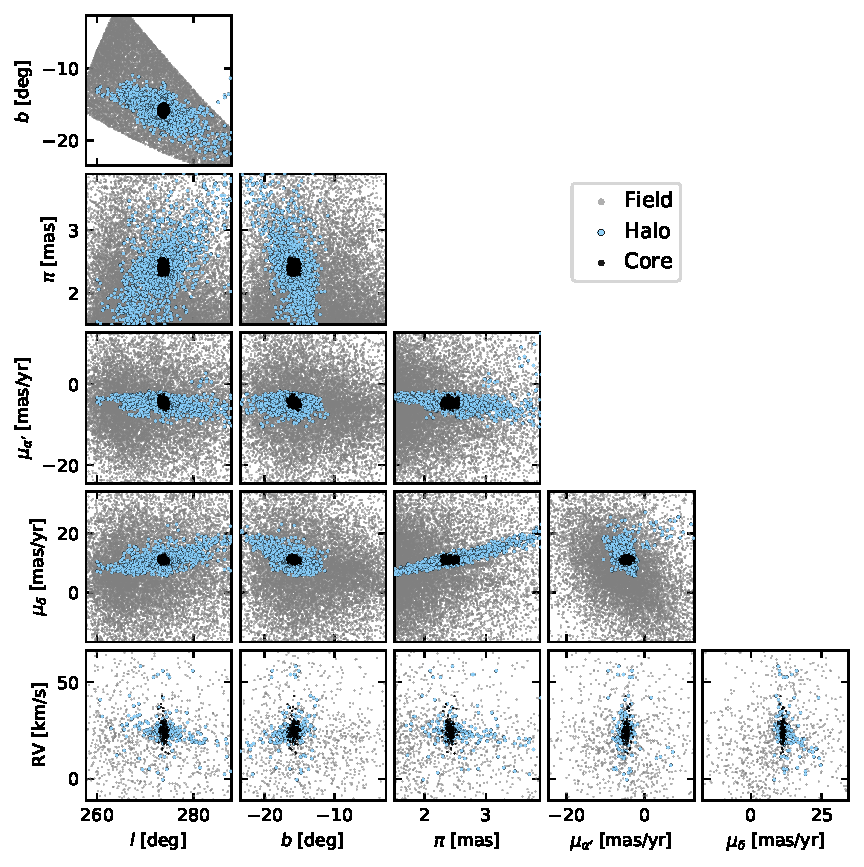
\includegraphics[width=0.95\textwidth]{f1.pdf}
	\end{center}
	\vspace{-0.7cm}
  \caption{ {\bf The dense and diffuse components of NGC\,2516 across
  position and velocity space.} The core (black) was analyzed by
  \citet{cantatgaudin_gaia_2018} using Gaia DR2, and is coincident
  with the visual overdensity of stars canonically accepted as ``the
  cluster''.  The halo (blue) is a concatenation of studies by
  \citet{kounkel_untangling_2019} and \citet{meingast_2021}, which
  used less restrictive membership assignment algorithms described in
  Appendix~\ref{app:clustering}.  The field sample is randomly drawn
  from a $(\alpha, \delta, \pi)$ cube centered on the cluster.  The
  low volume density of the halo stars makes it difficult to visually
  distinguish the field and the halo samples.
  \label{fig:gaia6d}
	}
\end{figure*}

\begin{figure*}[t]
	\begin{center}
		\leavevmode
		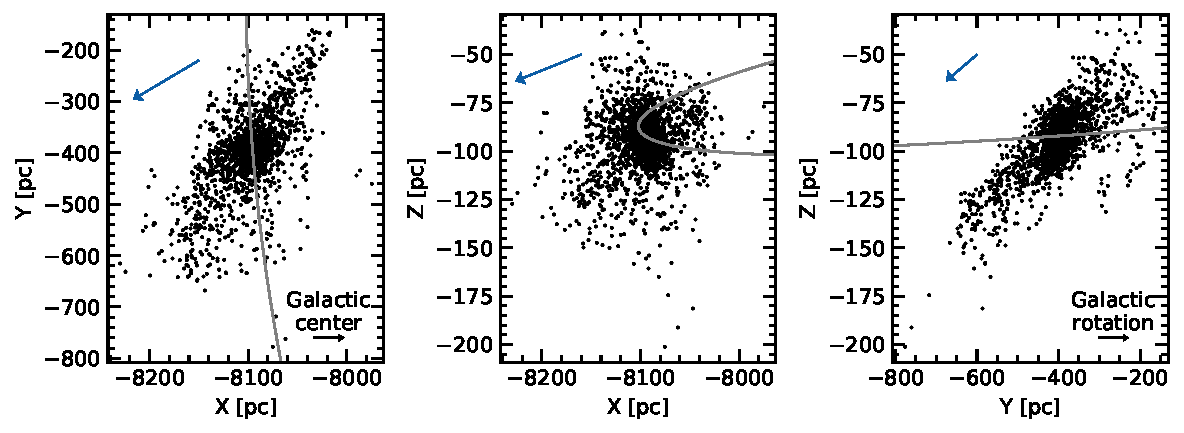
\includegraphics[width=0.95\textwidth]{f11.pdf}
	\end{center}
	\vspace{-0.7cm}
  \caption{ {\bf Position and orbit of NGC\,2516 in the Galaxy.}
  Points denote halo members with $\pi/\sigma_\pi>20$.  In our
  galactic coordinate system, the Sun is at $\{X,Y,Z\} = \{ -8122, 0,
  +20.8\}\,{\rm pc}$.  The gray line traces the past and future
  cluster orbit.  In different projections, the gray line spans
  different time intervals: the longest time window is visible in the
  $(Z,X)$ projection.  The large blue arrows denote the median cluster
  velocity after subtracting the local standard of rest: $\{v_{\rm X},
  v_{\rm Y}, v_{\rm Z}\} = \{-22.2, -25.3, -4.6\}$\kms.   By
  comparison, $\vec{v}_{\rm LSR} = \{12.9, 245.6, 7.78\}$\kms; in the
  inertial frame of the Galaxy, \cn\ is moving mostly in the $\hat{Y}$
  direction.  The sizes of the blue arrows are internally
  proportionate. 
  \label{fig:XYZ}
	}
\end{figure*}

We selected candidate \cn\ members based on those reported in the
literature.  While some pre-Gaia analyses were available
\citep{jeffries_ngc2516_2001,Kharchenko_et_al_2013}, the purity and
accuracy of the Gaia-derived results are the current state of the art.
We therefore adopted what we viewed as the most important Gaia-based
samples to compare: those of \citet{cantatgaudin_gaia_2018},
\citet{kounkel_untangling_2019} and \citet{meingast_2021}.  We refer
to these studies in the following as
\citetalias{cantatgaudin_gaia_2018},
\citetalias{kounkel_untangling_2019}, and \citetalias{meingast_2021}
respectively.  A useful visualization of these samples is
available online\footnote{
  \url{https://homepage.univie.ac.at/stefan.meingast/coronae.html},
  made by \citet{meingast_2021}, last accessed \texttt{2021/04/05}.}.
%While we considered performing our own clustering analysis on the
%Gaia data, such an effort would in effect only replicate the work of
%these investigators.  We opt to instead use their studies as a starting
%point.

The Gaia clustering studies each used different selection functions,
which yielded different results.  \citetalias{cantatgaudin_gaia_2018}
considered stars brighter than $G=18$\,mag within a few degrees of the
center of \cn, and reported 1106 candidate cluster members.
\citetalias{kounkel_untangling_2019} and \citetalias{meingast_2021}
considered stars up to $\approx$1\,mag fainter, and reported 3003 and
1860 members respectively.  The unsupervised clustering techniques
that each of these studies applied to the second Gaia data release are
discussed in Appendix~\ref{app:clustering}, as is the overlap between
their resulting membership catalogs.

Figure~\ref{fig:gaia6d} shows the cluster members reported by each
study in the space of observed positions, proper motions, and radial
velocity when available.
In Figure~\ref{fig:gaia6d}, and for the remainder of the study, we
describe the \citetalias{cantatgaudin_gaia_2018} members as the
``core'' of the cluster, and any non-overlapping
\citetalias{kounkel_untangling_2019} and \citetalias{meingast_2021}
members as the ``halo''.  This defintion implies that there are
\ncore\ core members, and \nhalo\ halo members.  The distinction is
tautological, in the sense that \citetalias{cantatgaudin_gaia_2018} did
not extend their search for members out to tens of degrees from the
cluster center.  Nonetheless, the \citetalias{cantatgaudin_gaia_2018}
membership catalog is consistent with that of many earlier
investigators \citep[{\it
e.g.},][]{jeffries_ngc2516_2001,Kharchenko_et_al_2013}, and is
consistent with the general visual overdensity one sees when viewing
\cn\ in the sky: it appears to span $\approx$2$^\circ$, not
$\approx20^\circ$.

Outside of the core and halo, we also define a set of nearby field
stars in the ``neighborhood'' of \cn.  Based on the observed
distribution of halo members, we drew these stars randomly from the
following intervals of right ascension, declination, and parallax:
\begin{align}
  \alpha\,[\mathrm{deg}] &\in [108, 132], \\
  \delta\,[\mathrm{deg}] &\in [-76, -45], \\
  \pi\,[\mathrm{mas}] &\in [1.5, 4.0].
\end{align}
We imposed a magnitude limit of $G=19$\,mag, and ran the queries using
the \texttt{astroquery.gaia} module \citep{astroquery_2018}.  We
allowed the number of stars in the comparison sample to exceed that in
the cluster sample by a factor of $\approx$5, to ensure broad sampling
of stellar masses and evolutionary states.  We also required the
comparison sample to not overlap with the cluster sample.

The style of visualization given in Figure~\ref{fig:gaia6d} does not
make it clear, in our eyes, why the clustering algorithms have decided
to associate certain stars with the halo.  Canonically, open clusters
are spherical, and span $\approx$10\,pc \citep[{\it
e.g.},][]{Kharchenko_et_al_2013}.  Inverting the parallaxes in
Figure~\ref{fig:gaia6d} shows that members have been reported from
line-of-sight distances ranging from $\approx$$300$ to
$\approx$$600\,$pc.  Is this structure real? What explains its
existence?

An initial step in visualizing the reported structure and kinematics
of the candidate cluster members is to consider their Cartesian
coordinates (Figure~\ref{fig:XYZ}).  We computed these positions by
transforming from $(\alpha, \delta, \pi)$ to galactic ($X,Y,Z$)
assuming the \texttt{astropy v4.0} coordinate standard
\citep{astropy_2018}.  The direction of galactic rotation is
$+\hat{Y}$. The cluster orbit (gray line) was evaluted by taking the
median parameters for core members for which
\citetalias{cantatgaudin_gaia_2018} reported membership probabilities
exceeding 70\%.  We then integrated the orbit using \texttt{gala} and
the \texttt{MWPotential2014} potential \citep{bovy_galpy_2015,gala}.

The general shape of the cluster itself seems to include a central
overdensity and two tails (the halo).  One tail is leading the
cluster's orbit, and is angled toward the center of the galaxy when
viewed top-down.  The other tail is trailing the cluster's orbit, and
is pointed away from the center of the galaxy.  The elongation of the
cluster in both the $(X,Y)$ and $(Z,Y)$ planes is correlated with the
direction of the LSR-corrected median cluster velocity.   Possible
explanations for this overall morphology are discussed in
Section~\ref{subsec:origin}.



\section{Age-Dating the Halo of NGC\,2516}
\label{sec:agedate}

\subsection{HR Diagram from Gaia}
\label{subsec:hr}

\begin{figure*}[t]
	\begin{center}
		\leavevmode
		\subfloat{
			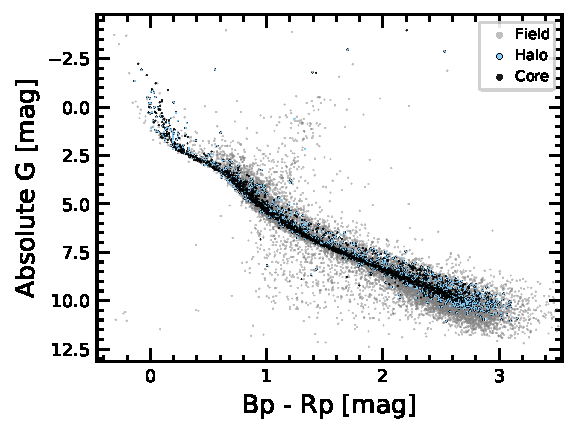
\includegraphics[width=0.49\textwidth]{f2a.pdf}
			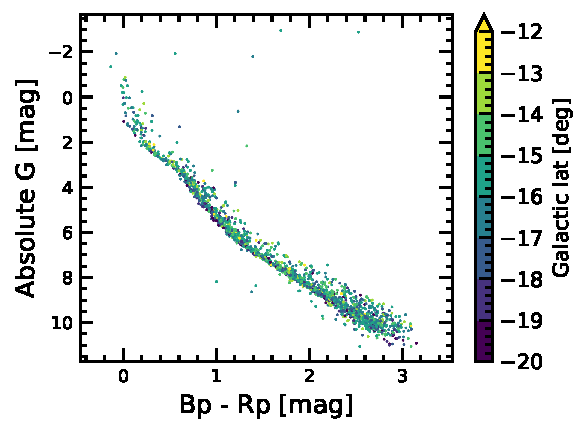
\includegraphics[width=0.49\textwidth]{f2b.pdf}
		}
	\end{center}
	\vspace{-0.7cm}
  \caption{ {\bf HR diagrams of NGC\,2516.}
    {\it Left}: Photometric data from Gaia EDR3; no reddening
    correction has been applied.  The core (black) shows a
    main-sequence and turnoff consistent with stars of a fixed age and
    metallicity.  The halo (blue) is similar, though the binary
    sequence is less defined.  The faintest M dwarfs in the core and
    halo are brighter than field stars (gray) with the same color,
    consistent with the cluster M dwarfs not having yet reached the
    main-sequence.  {\it Right}: PARSEC isochrones ([Fe/H]=+0.06) are
    overplotted at intervals of $\log_{10}(t/\mathrm{yr})=\{8, 8.25,
    8.5\}$.  The arrow represents the average reddening correction
    applied to the models.  The opacity of the M-dwarf model
    atmospheres is less well-calibrated for $M_\star \lesssim
    0.45M_\odot$ ($\approx$M2V; $\mathrm{Bp}-\mathrm{Rp}\approx$2.2);
    these model values are shown with dashed lines.
    \label{fig:hr}
  }
\end{figure*}

The first check on whether the candidate cluster members share the
same age is to analyze the Gaia Hertzsprung-Russell (HR) diagrams.
Comparable analyses have previously been performed by
\citetalias{cantatgaudin_gaia_2018},
\citetalias{kounkel_untangling_2019}, and \citetalias{meingast_2021}.

Figure~\ref{fig:hr} shows the HR diagram in the space of absolute Gaia
$G$ magnitude as a function of observed $\mathrm{Bp}-\mathrm{Rp}$
color.  Stars in the core appear consistent with having a fixed age
and metallicity, and varying mass.  The halo stars show a similar
sequence, though with greater scatter.  One possible explanation for
the additional scatter is that the halo is more contaminated by
field stars.  For instance, $\approx5$ red giants in the halo must be
field interlopers, because their isochronally implied ages would be
inconsistent with that of the cluster.

Another possible explanation for scatter in the halo's HR diagram
is differential reddening across different sightlines.  The
reported halo spans 20$^\circ$ on-sky, and varies in position from
about $b=-12^\circ$ to $b=-20^\circ$, with the stars closest to the
galactic plane also being further from the Sun by up to 300\,pc
(Figure~\ref{fig:gaia6d}).  An HR diagram binned by galactic latitude
did show some minimal evidence for differential reddening, and so we
expect that both field star contamination and differential reddening
could play a role in the larger scatter of the halo relative to the
core.  A third possibility that we have not explored is whether the
binary fraction could also differ between the different regions of the
cluster.

In the right panel of Figure~\ref{fig:hr}, we compare the observed
Gaia EDR3 photometry with PARSEC isochrones
\citep{bressan_parsec_2012,chen_improving_2014,chen_parsec_2015,marigo_new_2017}.
We used the web
interface\footnote{\url{http://stev.oapd.inaf.it/cgi-bin/cmd},
\texttt{2021-02-26}, \texttt{CMD3.4}, \texttt{YBC} bolometric
corrections as in \citet{chen_2019_YBC}.} to interpolate these
isochrones at $\log_{10}(t/\mathrm{yr})=\{8, 8.25, 8.5\}$.

To determine the reddening correction across \cn, we queried the 2MASS
DUST service\footnote{
  \url{http://irsa.ipac.caltech.edu/applications/DUST}; query
  performed using the \texttt{astrobase.services.dust} module
  \citep{bhatti_astrobase_2018}.  } and retrieved the total
line-of-sight extinction parameters at the positions of each \cn\ 
member.  The mean and standard deviation of the
$E(\mathrm{B}-\mathrm{V})$ values for the \citet{schlegel_maps_1998}
and \citet{schlafly_measuring_2011} maps were consistent, so we
adopted the average from \citet{schlegel_maps_1998}:
$E(\mathrm{B}-\mathrm{V})_{\rm S}=0.206\pm0.039$.
\citet{bonifacio_search_2000} found however that the
\citet{schlegel_maps_1998} maps overestimate the reddening values when
the color excess exceeds about 0.10\,mag. We therefore applied the
correction proposed by \citet{bonifacio_search_2000}, and additionally
corrected for the mean cluster distance by a factor
$\exp(-|d\sin(b)|/h)$ where $d$ is the average cluster distance,
$b$ is the average galactic latitude, and $h$ is the scale height of
the galactic disk, assumed to be 125\,pc.  This yielded our adopted
$E(\mathrm{B}-\mathrm{V})=0.102\pm0.019$, where the uncertainty
reflects the standard deviation of the individual
\citet{schlegel_maps_1998} values.  Finally, to convert to Gaia
colors we used the calibration of \citet{stassun_TIC8_2019}, namely
$E(\mathrm{Bp}-\mathrm{Rp})=1.31 E(\mathrm{B}-\mathrm{V})$ and
$A_G=2.72 E(\mathrm{B}-\mathrm{V})$.  This yielded
$E(\mathrm{Bp}-\mathrm{Rp})=0.134\pm0.025$, which is used in the
plots.  To redden the isochrones, we assumed $R_V=3.1$, and applied
the \citet{odonnell_1994} SED-dependent extinction law star-by-star
through the PARSEC interface. 

For the metallicity, we considered a range of super and sub-solar
metallicities to fit as much of the locus from
$0.5<\mathrm{Bp}-\mathrm{Rp}<1.5$ as possible, and settled on the
slightly super-solar $[M/H]=0.06$ \citep{cummings_2011_li_iron}.
Sub-solar metallicities led to model predictions too blue along the
main sequence by $\approx$0.1\,mag.  Our adopted metallicity agrees
with the spectroscopic metallicity from
\citet[][Sec~4.4.4]{cummings_2011_li_iron}, and with the iron
abundance recently determined by the Gaia-ESO team
\citep{baratella_gaiaeso_2020}, which represented an up-revision from
an earlier sub-solar metallicity \citep{randich_gaiaeso_2018}.  We
caution though that other sub-solar metallicities have been reported
\citep{bailey_rv_2018}, and note that the cluster metallicity and
reddening are degenerate; if the reddening is lowered, the implied
metallicity will increase.  While a detailed redetermination of
these parameters from the Gaia photometry is beyond our scope, our
adopted values for both the reddening and metallicity are within the
range of previously reported values in the literature.

Overall, the data and models agree for masses above
$\approx$0.45\,$M_\odot$.  Below this mass, the data and models
diverge at colors redder than $\mathrm{Bp}-\mathrm{Rp}\approx2.2$, in
the sense that the model isochrones have lower luminosities and bluer
colors than the observations.\footnote{The 100 Myr isochrone does
overlap well with the lower main sequence, but it fails to fit the
upper main sequence and red giants.}  The MIST isochrones showed a
comparable disagreement \citep{choi_mesa_2016}.  Proposed explanations
for the discrepancy between the models and observations have include
starspots and incomplete molecular line lists\citep[{\it
e.g.},][]{stauffer_why_2003,feiden_magnetic_2013,rajpurohit_effective_2013,mann_spectrothermometry_2013,choi_mesa_2016}.
Ultimately, we adopted the PARSEC isochrones because
\citet{chen_improving_2014} implemented an empirical
temperature-opacity calibration, which leads the PARSEC isochrones to
diverge at slightly lower mass than the MIST models.  Regardless, for
purposes of age-dating the cluster we focus on the main-sequence
turn-off (MSTO), since this is where the models have maximum
sensitivity to age.

\citet{cummings_2018} presented techniques for mitigating some of the
complexities of MSTO age-dating ({\it e.g.}, sparse turnoffs, stellar
rotation, high binarity fractions, and the presence of blue
stragglers).  Combining a $UBV$ color-color analysis with Gaia DR2
cluster memberships, they found MSTO ages for NGC\,2516 ranging from
165 to 195\,Myr, depending on the choice of model isochrone (Y$^2$,
PARSEC, MIST, or SYCLIST).

Our goal is to determine whether the ages of the core and halo are
consistent.  The left panel of Figure~\ref{fig:hr} suggests that
isochronally, they are consistent: stars past the turnoff in both the
halo and core are on the same locus.  The right panel of
Figure~\ref{fig:hr} demonstrates the precision with which the claim
can be made.  The MSTO stars are consistent with the 178 and 316 Myr
models, but are bluer than the 100 Myr model.  The red-giant-branch
(RGB) stars are consistent only with the 178 Myr ($\log_{10} t/{\rm
yr} = 8.25$) model.  Based on the assumption that the width of the
MSTO can be attributed to binary stars, we are most interested in the
blue edge (blue stragglers are, however, a concern).  The blue edge
appears most compatible with the 178 Myr model.  These results are
consistent with the MSTO age range of 165 to 195\,Myr found by
\citet{cummings_2018}, and we refer to their work for the more precise
model-dependent comparison.  Based on Table~3 of
\citet{cummings_2018}, we therefore adopt a MSTO age for \cn\ of
$175\pm35$\,Myr, where our quoted uncertainty is a quadrature sum of
the statistical and systematic components from \cite{cummings_2018}. 



\subsection{Rotation from TESS}
\label{subsec:tess}

\subsubsection{Methodology}
\label{subsubsec:cluster}

\begin{figure*}[t]
	\begin{center}
		\leavevmode
		\subfloat{
			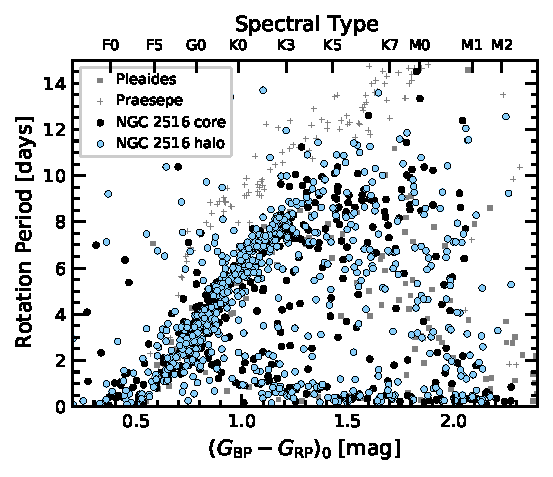
\includegraphics[width=0.49\textwidth]{f3a.pdf}
			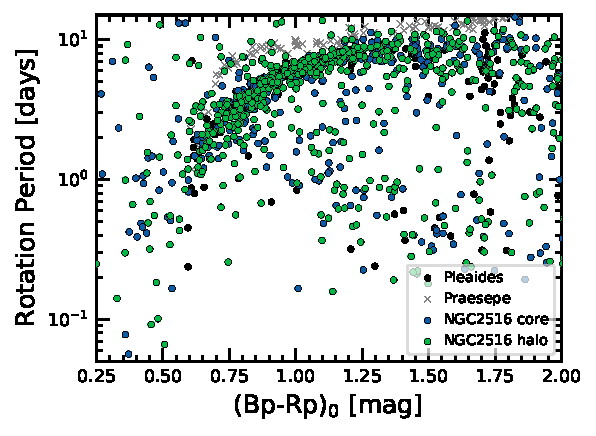
\includegraphics[width=0.49\textwidth]{f3b.pdf}
		}

        \vspace{-0.5cm}
		\subfloat{
			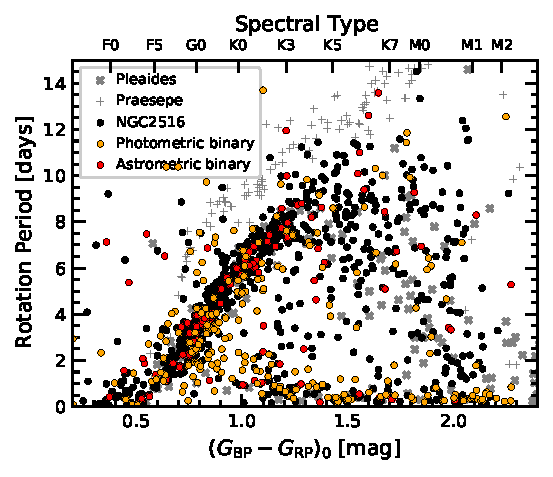
\includegraphics[width=0.49\textwidth]{f3c.pdf}
			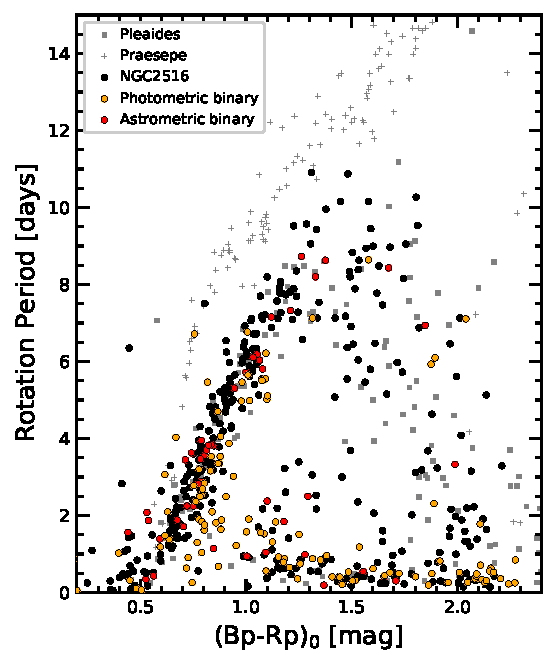
\includegraphics[width=0.49\textwidth]{f3d.pdf}
		}
	\end{center}
	\vspace{-0.7cm}
  \caption{ {\bf TESS rotations periods and dereddened Gaia colors for
  \cn.} {\it Top row}: \cn\ split into its core and halo.  Sets
  $\mathcal{A}$ ({\it left}) and $\mathcal{B}$ ({\it right}) undergo
  successive stages of automated cleaning, (see
  Section~\ref{subsubsec:cluster}).  The Pleiades
  \citep[125\,Myr;][]{rebull_rotation_2016a} and Praesepe
  \citep[650\,Myr;][]{douglas_poking_2017} are shown for reference.
  Stars in the core and the halo of NGC\,2516 overlap with the
  Pleiades at $\bpmrp$$<$1.2.  From $1.2<\bpmrp<1.7$, some NGC\,2516
  members have longer rotation periods than Pleaides members.  {\it
  Bottom row}: \cn\ colored by binarity indicators.  Sources with
  $\mathrm{RUWE}>1.2$ appear in red (astrometric binaries; 11\% of
  stars).  Overplotted in orange are sources at least 0.3\,mag above
  an empirically fit cluster isochrone (photometric binaries; 20\% of
  stars).
  Rotation periods for comparison field stars are shown in
  Appendix~\ref{app:compstar}.
  \label{fig:rot}
	}
\end{figure*}

We began our rotation analysis by considering all \nkinematic\
candidate members of \cn.  For each source, we retrieved all available
CDIPS light curves, on a per-sector basis.  This yielded \ncdips\
stars with at least one sector from a CDIPS light curve.  Each of
these stars is brighter than the CDIPS magnitude limit of
$Rp=16$\,mag.  \nkinematicrpltsixteen\ of the stars from the \cn\
source list had $Rp<16$.  The difference (65 stars) is due to 35 stars
from \citet{meingast_2021} which were not available at the time of the
CDIPS reductions, and 30 stars falling on the TESS chip gaps.  At the
distance of \cn, the $Rp=16$\,mag cutoff imposed during the CDIPS
processing corresponds roughly to $\bpmrp$ of 2.2, or a spectral type
of $\approx$M2V.

We removed systematic trends shared between all light curves on each
CCD in each sector individually, and stitched together the resulting
light curves before searching for rotation-induced periodicity.
Details regarding our detrending approach are presented in
Appendix~\ref{app:detrending}.  After detrending, we proceeded with a
few cleaning steps: we masked 0.7 days at the beginning and end of
each spacecraft orbit, and ran a sliding standard-deviation rejection
window over the light curve, which removed any outlying points within
$\pm3\times$MAD of the median in each window.

We then measured the rotation period from the resulting light curve
using the periodogram implementations in \texttt{astrobase}, namely
the traditional Lomb-Scargle, and the Stellingwerf phase-dispersion
minimization algorithm
\citep{lomb_1976,stellingwerf_period_1978,scargle_studies_1982,stellingwerf_period_2011,bhatti_astrobase_2018}.
We used the CDIPS aperture radius that, based on theoretical
expectations, was expected to give the optimal balance between light
from the target star and background-light \citep{Sullivan_2015}.  This
typically resulted in a circular aperture radius of either 1 or 1.5 pixels.
We recorded the top five periodogram peaks from each method, and their
corresponding powers.  Finally, as a check on crowding, we recorded
the number of stars within the aperture with equal or greater
brightness than the target star, and with brightness within 1.25 and
2.5 TESS magnitudes of the target star.

The resulting rotation periods and periodogram powers are reported,
regardless of detection significance, in Table~\ref{tab:maintable}.
To clean the resulting rotation period measurements, we designed a set
of automated cleaning criteria, which yielded sets we denote
$\mathcal{A}$ and $\mathcal{B}$.  For both sets, we considered light
curves for which the peak Lomb-Scargle periodogram period was below 15
days, the normalized Lomb-Scargle power exceeded 0.08, and for which
no equal-brightness or greater companions were within the aperture.
These limits were chosen after inspecting the light curves visually,
to eliminate low-quality rotation periods while retaining high
completeness.  Beyond requiring that the target star be the brightest
star in the aperture, we also required that at most one companion with
brightness exceeding one tenth of the target star's brightness be
present in the aperture according to the Gaia DR2 source catalog.  For
set $\mathcal{A}$, this yielded \nautorotnumerator\ light curves, out
of \nautorotdenominator\ stars for which rotation periods might
plausibly have been detected.  For set $\mathcal{B}$, we additionally
required that the Lomb-Scargle and Stellingwerf phase-dispersion
methods yielded identical periods to within 10\%.  This yielded
\nautorotnumeratormatching\ light curves.  Boolean flags for each set
are included in Table~\ref{tab:maintable}.

\subsubsection{Rotation-Color Diagrams}

The top row of Figure~\ref{fig:rot} shows the resulting rotation
periods, with set $\mathcal{A}$ shown the left and $\mathcal{B}$ on
the right.  While set $\mathcal{A}$ is more complete than set
$\mathcal{B}$, this completeness comes at the expense of greater
contamination.  For instance, stars above the slow sequence (perhaps
field contaminants) mostly disappear in set $\mathcal{B}$.  The
``void'' or ``gap'' underneath the slow sequence is also more
pronounced in set $\mathcal{B}$.  To facilitate a comparison against
the Pleiades and Praesepe, we used the rotation periods and dereddened
colors from Table~5 of \citet{curtis_rup147_2020}, which drew on data
from \citet{rebull_rotation_2016a} and \citet{douglas_k2_2019}
respectively.  The first order conclusion is that the Pleiades and
\cn\ appear gyrochronologically coeval for colors spanning
$0.5<\bpmrp<1.2$.  The implications of this comparison for the age of
\cn\ are discussed in Section~\ref{disc:absage}.

The bottom row of Figure~\ref{fig:rot} shows the same data, with the
points colored with indicators of binarity.  To assess astrometric
binarity, we used the renormalized unit weight error (RUWE) from Gaia
EDR3.  For plotting purposes, we labeled anything with RUWE exceeding
1.2 as an astrometric binary (11\% of the overall cluster sample; see
{\it e.g.}, \citealt{belokurov_unresolved_2020}).  To assess
photometric binarity, we fitted a spline to Figure~\ref{fig:hr},
fixing the nodes by hand.  We then labeled any points brighter than
0.3\,mag above the cluster sequence as photometric binaries.  This
included 20\% of the overall cluster sample.  Many of the resulting
candidate binaries, though not all of them, appear below the slow
rotation sequence.  In set $\mathcal{B}$, over the color range where
the slow and fast sequence are present ($0.5<\bpmrp<1.3$), there are
281 stars, of which 103 (37\%) show signs of binarity.  Dividing these
281 stars into ``fast'' and ``slow'' sequences by eye,  the fraction
of stars showing signs of binarity in the slow and fast subsamples are
30\% (63/210) and 56\% (40/71), respectively.  We speculate on
possible explanations in Section~\ref{disc:rotn}.


\subsubsection{Comparing Kinematics and Rotation}

\begin{figure*}[t]
	\begin{center}
		\subfloat{
			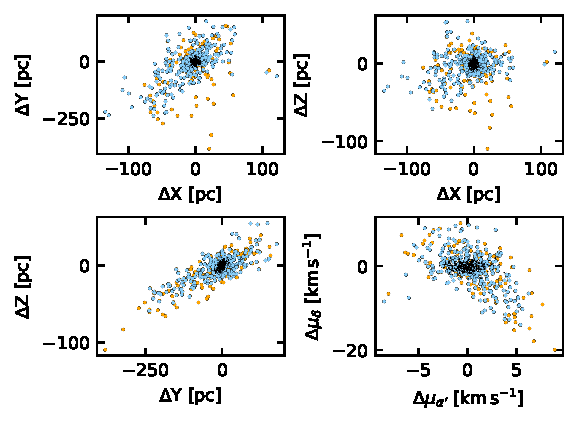
\includegraphics[width=0.48\textwidth]{f8a.pdf}
			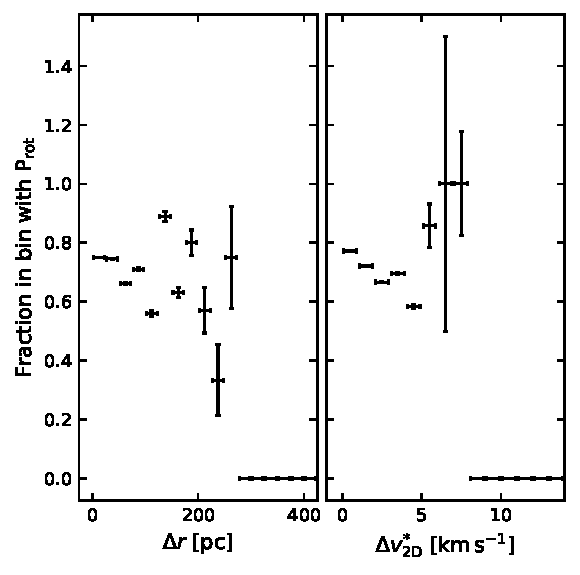
\includegraphics[width=0.5\textwidth]{f8b.pdf}
		}

		\subfloat{
			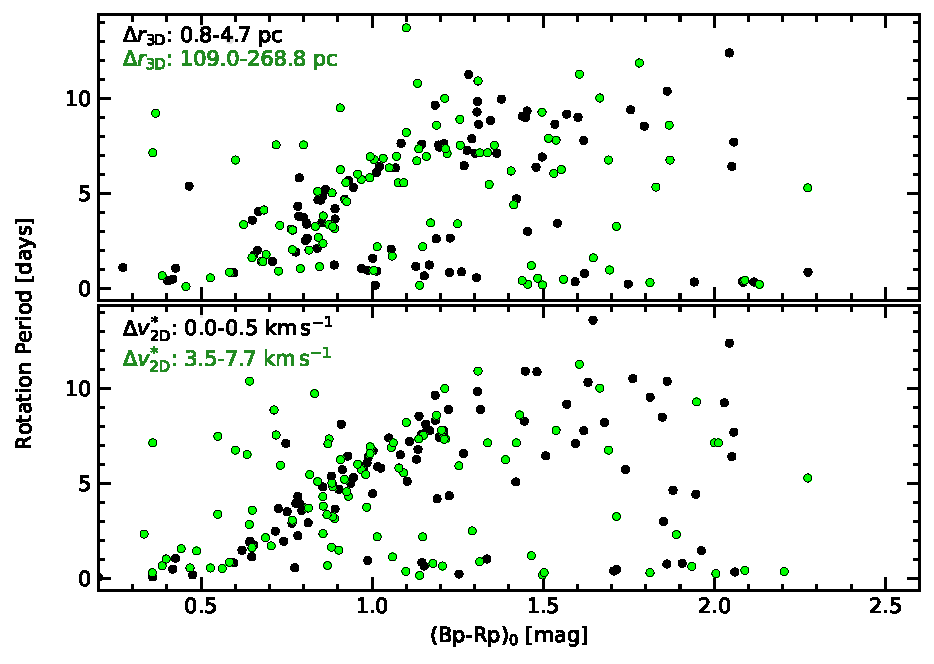
\includegraphics[width=0.9\textwidth]{f13.pdf}
		}

	\end{center}
	\vspace{-0.7cm}
  \caption{ 
  {\bf \cn\ members exist hundreds of parsecs from the core, and up
  to $\approx$5\kms\ from the core in tangential velocity.} {\it Top
  left}: Cartesian positions (as in Figure~\ref{fig:XYZ}) and
  2D-tangential velocities for halo members that meet kinematic
  membership criteria (Subset~$\mathcal{A}$).  Stars with detected
  rotation periods are shown in blue;  halo members for which rotation
  periods should have been detectable, but were not detected, are
  shown in orange.  Stars in the core are shown as black points.
  Computing the 2D-tangential velocity requires correcting for
  projection effects (Appendix~\ref{app:vproj}).  In the {\it top
  right}, the histograms on bin versus 3D separation from the core and
  2D tangential velocity difference.  Bin widths are chosen to enforce
  the same number of stars in the denominator ($N=54$) per bin.  In the
  {\it bottom panels}, the innermost and outermost 100 stars in
  position and velocity space (black and green) are shown in the
  space of rotation periods and dereddened colors.
  \label{fig:physical_x_rotn}
	}
\end{figure*}

The TESS rotation periods provide an independent check on the
Gaia-derived kinematic cluster memberships.  We explored this by
cross-matching the stars with detected TESS rotation periods against
our original target list of \nkinematic\ Gaia members.  

To visualize the results, we again opted for Cartesian coordinates,
and supplemented them by calculating the tangential stellar velocities
relative to the cluster center.  Appendix~\ref{app:vproj} discusses
the projection effect correction required for calculating the
tangential velocities: for a star at position $(\alpha, \delta)$, we
compare the observed proper motion $(\mu_{\alpha'}, \mu_\delta)$ with
what the proper motion at the star's position would have been if the
star were comoving with the core of \cn.  This yields a quantity we
denote $\Delta v^{*}$, per \citetalias{meingast_2021}.  We convert
these proper motion differences to physical units by multiplying by
the measured parallax.  

The results are shown in the top two rows of
Figure~\ref{fig:physical_x_rotn}.  In these figures, to ensure a fair
comparison, we only show stars with $0.5<\bpmrp<1.2$ for which our
TESS pipeline succeeding in making light curves.  In other words, the
stars in the base sample are those for which we could have plausibly
detected a rotation period.  This color range is preferred because the
the slow sequence becomes less defined for spectral types later than
$\approx$K4V.  The bins in the histograms (top-right) were chosen to
ensure that the same number of stars were in each bin.  Rotation
periods are detected for 66\% of stars at least 25\,pc from the
cluster core.  The average detection rate inside of 25\,pc, 73\%, is
slightly higher.  With $\approx$3.5\,pc, the period detection rate of
61\% is relatively low, due to the combined effects of crowding and
saturation.

The lower panels of Figure~\ref{fig:physical_x_rotn} give a second
view of how field star contamination affects the outskirts of the
cluster.  Of the outermost 100 stars in position space with detected
rotation periods, $\approx$8 appear as outliers above the slow
sequence, compared to just a few for the innermost 100 stars.  For the
outermost 100 stars in velocity space, $\approx$13 appear as outliers.
After accounting for the stars that were expected to show rotation
periods and did not, this suggests field contaminant rates of
$\approx$40-50\% for the outermost cluster members in our target list.

Even with this level of contamination, our rotation period
measurements show that the halo extends to separations of
$\approx$250\,pc in physical space from the cluster core.  The most
widely separated F2V-K2V stars with rotation periods (blue points in
Figure~\ref{fig:physical_x_rotn}) are separated by $\approx$430\,pc.
The total length of the structure is therefore 400--500\,pc, depending
on which members of the halo are chosen as the ``tips'' on either end.
This agrees with the overall structure of the halo reported by
\citetalias{kounkel_untangling_2019}, with some minor caveats visible
in the top-left panels of Figure~\ref{fig:physical_x_rotn}.

In projection-corrected tangential velocity space, the fraction of
stars with rotation period detections remains high out to roughly
5\kms.  \citet{meingast_2021} by comparison required a physically
motivated cut in tangential velocity space of 1.5\kms.  Our results
show that at the expense of higher field star contamination rates,
bonafide members can be identified even out at higher velocity
separations.


\subsection{Lithium from Gaia-ESO and GALAH}
\label{subsec:lithium}

\begin{figure*}[t]
	\begin{center}
		\leavevmode
			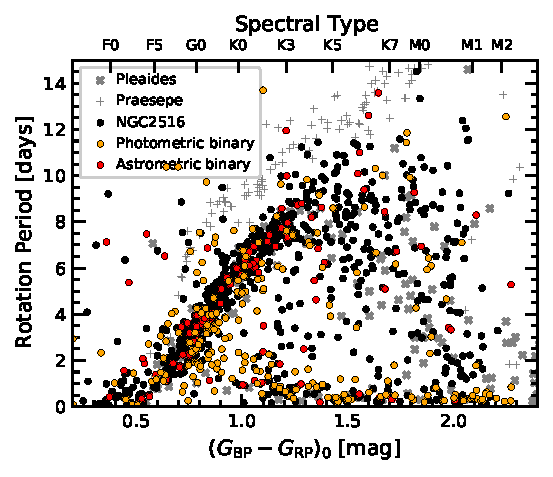
\includegraphics[width=0.9\textwidth]{f5a.pdf}
	\end{center}
	\vspace{-0.7cm}
  \caption{ {\bf Lithium in the core and halo of NGC\,2516.}
  Equivalent width of the 6708\,\AA\ doublet is shown versus
  dereddened color for all kinematic \cn\ members with Gaia-ESO
  ($N=452$) or GALAH ($N=107$) spectra available.  The GALAH spectra
  comprise slightly over half of the halo stars, due to the
  non-targeted selection function of that survey.  Field stars (gray
  points) are Keck-HIRES measurements of stars with detected
  transiting planets from the Kepler mission
  \citep{berger_identifying_2018}.  Stars in the Pleiades (125\,Myr)
  with Li detections are from \citet{bouvier_pleiades_lirot_2018};
  Praesepe detections (650\,Myr) are shown in violet
  \citep{soderblom_praesepe_1993}.  Points with ${\rm
  EW}\approx0\,$m\AA\ are non-detections.
  The Li measurements for both Core and Halo stars in \cn\ are
  consistent with a near-Pleiades age.
  {\bf LGB TODO: the increasing EWs for the Gaia-ESO M dwarfs must be erroneous. What's happening there?}
  \label{fig:lithiumcorehalo}
  }
\end{figure*}
\begin{figure*}[t]
	\begin{center}
		\leavevmode
		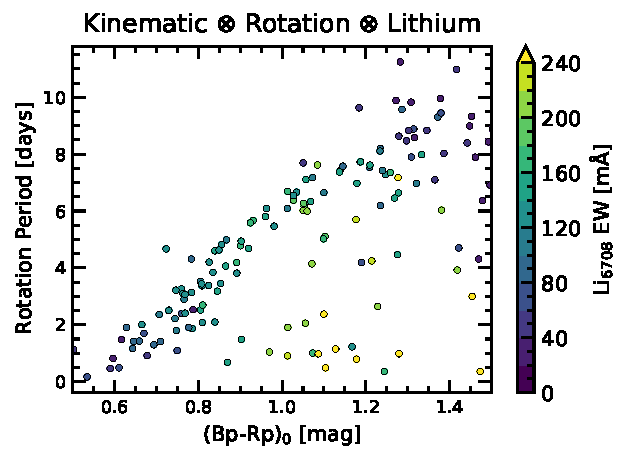
\includegraphics[width=0.9\textwidth]{f5b.pdf}
	\end{center}
	\vspace{-0.7cm}
  \caption{ {\bf Lithium and rotation in NGC\,2516.} Points show all
  kinematic \cn\ members with TESS rotation periods in the Gaia-ESO or
  GALAH surveys, and are colored by equivalent width.  Points with
  reported equivalent widths below 20\,m\AA\ (including
  non-detections) are shown with gray crosses.  The lithium-rotation
  correlation for the K-dwarfs has been observed in other young
  clusters, and is discussed in Section~\ref{subsec:lithium}.
	\label{fig:lithiumrot}
	}
\end{figure*}

The third and final approach we took for confirming the youth of the
halo population of \cn\ was an analysis of the Li\,\textsc{I}
6708\,\AA\ doublet.  This type of age measurement has been reviewed by
\citet{soderblom_ages_2010}, and its connection to stellar rotation
has recently been surveyed by \citet{bouvier_lithium-rotation_2020}.
For \cn, two spectroscopic datasets seemed important:
Gaia-ESO \citep{gilmore_gaiaeso_2012} and GALAH
\citep{silva_galah_2015}.  At the time of analysis, Gaia-ESO DR4 and
GALAH DR3 were the most relevant, respectively \citep[{\it
e.g.},][]{randich_gaiaeso_2018,buder_galah_2020}.  The target
selection and results from each survey were as follows.

Gaia-ESO selected candidate \cn\ members to observe with the GIRAFFE
and UVES spectrographs based on previously reported literature members
and publicly available photometry.  Since the existence of the \cn\
halo was not known at the time of target selection, very few halo
stars are in the sample.  For \cn, \citet{randich_gaiaeso_2018}
reported stellar parameters (including lithium equivalent
widths and metallicities) for 796 stars that they considered possible
\cn\ members.  Cross-matching against our kinematic list of
\nkinematic\ candidate members by position and imposing a 0$\farcs$5
maximum separation limit yields 492 kinematic members for which a
Gaia-ESO spectrum was acquired and stellar parameters were reported.
15 of these (all with $\bpmrp > 2.0$) are spurious matches based on
the Gaia color and GES effective temperature, and we remove them.
This yields 477 stars, of which 436 are in the core, and 41 are in the
halo.  The lop-sided ratio is due to the Gaia-ESO selection function.
We verified by directly querying the ESO archive that
\citet{randich_gaiaeso_2018} indeed included $>99\%$ of the available
Gaia-ESO spectra as part of their \cn\ sample, and so we opted to use
their results rather than repeating their analysis.

The GALAH DR3 target selection is discussed in depth by
\citet{buder_galah_2020}.  The relevant aspects for our analysis are
that the ``main'' survey targeted $12<V<14$ stars at
$\delta<+10^\circ$, provided the stars were at least ten degrees from
the galactic plane.  The survey is spatially
inhomogeneous\footnote{See the footprint at
\url{https://www.galah-survey.org/news/announcing-galah-dr3}}. Special
targeting for stars in the TESS southern continuous viewing zone, and
for known open cluster members was also performed.  We identified the
candidate \cn\ members for which spectra had been obtained by
searching the \texttt{GALAH\_DR3\_main\_allstar\_v1} catalog, after
excluding stars with the stellar parameter bit flags 1, 2, 3.  This
excludes spectra with unreliable broadening, low S/N, and unreliable
wavelength solutions (see Table~6 of \citealt{buder_galah_2020}).
Since our main focus is measuring equivalent widths for the
Li\,6708\,\AA\ doublet, these were the most relevant bit flags.  Of
our \nkinematic\ candidate \cn\ members, 107 had spectra in GALAH DR3.
51 were in the ``core''; 56 were in the ``halo''.  78 had ``finite''
lithium, i.e., no lithium flag set.

%
%/Users/luke/Dropbox/proj/earhart/results/lithium/kinematic_X_galah_dr3.csv
% https://docs.datacentral.org.au/galah/dr3/catalogue-data-access/
%

We downloaded\footnote{Via \url{datacentral.org.au/services/download},
using the \texttt{sobject\_id} identifiers.} the GALAH DR3 spectra for
all 107 entries.  We then measured the lithium equivalent widths using
the \texttt{specutils} package \citep{specutils_v1pt1}.  We did this
by first focusing in on a 15\AA\ window centered on the 6707.835\AA
lithium doublet.  We then continuum normalized the spectra using a
third-degree Chebyshev series, while excluding any regions that showed
absorption lines ({\it e.g.}, Fe\,\textsc{I} is present at
6703.58\,\AA and 6705.10\,\AA).  We proceeding by fitting a Gaussian
to the continuum normalized spectra, considering only a $\pm 1\,$\AA\ 
window centered on the Li doublet.  The equivalent widths were then
evaluated by numerically integrating the fitted model over the same
window.  Our approach therefore includes the Fe\,6707.44 blend in the
reported Li equivalent widths---which leads to systematic
overestimates of $\approx$10 to 15\,m\AA\ \citep[{\it
e.g.},][]{bouvier_pleiades_lirot_2018}.  Finally, to derive
uncertainties on the EWs, we repeated the procedure twenty times, but
added noise to the spectra, drawn from a normal distribution with a
scale set by the standard deviation of the continuum.  The reported
uncertainties are then drawn from the $84^{\rm th}$ and $16^{\rm th}$
percentiles of the resulting EW distribution.  We verified the overall
scale of our results by comparing the 21 stars that overlapped between
GALAH and Gaia-ESO.  17 of the 21 measurements agreed within
1-$\sigma$.  The remaining four were stars with $T_{\rm
eff}>6200\,{\rm K}$, for which \citet{randich_gaiaeso_2018} reported
Li EW detections ranging from $50$ to $75\,$m\AA, and for which we
found either null results or only slightly significant
($\approx$30m\AA) detections.

% The outliers:
%    Fitted_Li_EW_mA     EWLi            source_id  Teff
%    24           -1.490   76.100  5290730488348194304  6786
%    34           19.485   71.300  5290935341107132800  6702
%    15           20.251   50.867  5290722310730727040  6197
%    25           29.378   52.500  5290724681552584192  6511

Figure~\ref{fig:lithiumcorehalo} shows the concatenation of the
Gaia-ESO and GALAH results, with the points colored according to whether the
stars are in the core or the halo of the cluster.  The GALAH spectra
span a color range of $0<\bpmrp<1.5$, due to the $V<14$ brightness
cutoff of the survey.  The overall increase of Li EW from
$0<\bpmrp<1.0$ is driven by the temperatures in the stellar
chromospheres: hotter stars fully ionize Li out of its ground state
\citep[{\it e.g.}, Figure~4 of][]{soderblom_evolution_1993}.  The
depletion of stars redder than $\bpmrp\gtrsim1.4$, {\it i.e.}, later
than K4.5V (0.71\,$M_\odot$), is visible relative to the earlier K
dwarfs: these stars have burned their lithium.  For comparison, we
have also plotted the Li EWs measured by
\citet{berger_identifying_2018} for planet-hosting stars in the Kepler
field, and Pleiades members from \citet{bouvier_pleiades_lirot_2018}
(we interpolated from their effective temperatures using the
\citet{pecaut_mamajek_2013}
table\footnote{\url{http://www.pas.rochester.edu/~emamajek/EEM_dwarf_UBVIJHK_colors_Teff.txt},
version 2021.03.02.}.  For clarity, we have omitted the few upper
limits reported by \citet{bouvier_pleiades_lirot_2018}.  The field
star distribution peaks at late F-type stars.  The majority of
kinematically selected stars in the core and the halo show lithium
equivalent widths substantially in excess of these field stars.

We can go one step further, and match our sample of kinematically
selected stars with spectra against the TESS rotators.  The result is
shown in Figure~\ref{fig:lithiumrot}. At fixed stellar mass, the rapid
rotators have lithium equivalent widths an order of magnitude larger
than the slow rotators.  This effect is mostly apparent in the K
dwarfs.  Similar trends were noted in the Pleiades over three decades
ago \citep{butler_pleiades_1987}, and are thought to be caused by
differences in lithium abundance
\citep{soderblom_evolution_1993}.  Alternative explanations, such as
differences in line-formation conditions ({\it e.g.,} chromospheric
temperatures, microturbulent velocities, or the presence of starspots)
are incompatible with the available data.  The lithium-rotation
correlation is discussed further below
(Section~\ref{discussion:lithium}).




\section{Discussion}
\label{sec:discussion}

\subsection{How did the halo form?}
\label{subsec:origin}

Any theory for the structure of \cn, the Psc\,Eri stream, and the
strings and halos found by \citetalias{kounkel_untangling_2019} and
\citetalias{meingast_2021} needs to explain a few observations.  First
is their aspect ratios.  The halo of \cn, for instance, extends over
at least 500\,pc, despite being only $\approx$25\,pc wide.  Second is
their axial tilts in the plane of the Milky Way -- why their leading
and trailing arms tend to conform to the Galaxy's differential
rotation ({\it e.g.}, Figure~\ref{fig:XYZ} or Figure~13 of
\citetalias{meingast_2021}).  Third is the correlation between the
mean LSR-subtracted cluster velocity and elongation axes (blue arrows
in Figure~\ref{fig:XYZ}).  Such a correlation has also been noted in
Coma Ber by \citet{tang_comaber_2019}; the other halos may show
similar trends.

One possible explanation is that the observed halo structures are
tidal tails \citep[{\it e.g.},][]{krumholz_star_2019}. The idea is
that as the cluster contracts, stars escape out of the Lagrange points
imposed by the Milky Way's potential, and form leading and lagging
arms due to differential rotation in the Galaxy.  Kinematic evidence
that the core of \cn\ may be undergoing contraction has recently been
presented by \citet{healy_stellar_2020}, which might increase the rate
at which stars escape.  Whether the exact contraction rate, and the
corresponding evaporation rate of the core are sufficient to
explain the formation of the halo has yet to be assessed.  The
presence or lack of epicyclic overdensities in the tails might also
help clarify whether this scenario is happening
\citep{kupper_more_2012}.

A second possibility is that the clusters form in larger and more
dispersed star formation complexes: the stars in the halo need not
have formed in the same ``clump'' as those in the cluster core.  In
other words, the formation environment might be better described a
giant molecular filament, rather than a giant molecular cloud.  A
sample of such filaments has recently been collected and analyzed by
\citet{zucker_physical_2018}: if the current $\approx$20:1 aspect
ratio of \cn\ were primordial, its structure would match the aspect
ratios of what they term either ``elongated dense core complexes'', or
``bone candidates''.  A more immediate example is the Orion\,A cloud.
\citet{grosschedl_3d_2018} showed using young stellar objects as
tracers that Orion\,A is 90\,pc long, and that it has a dense ``head''
and a lower density ``tail''.

One way to rule between the two possibilities would be to
observationally establish an age-size correlation.  If the
$\approx$100\,Myr halos are produced primarily through evaporation and
expansion, then the younger clusters should be significantly smaller.
A theoretical approach along similar lines would be to perform a
dynamical analysis of whether filaments like Orion\,A, or those in the
\citet{zucker_physical_2018} sample, are at all expected to evolve
into structures resembling \cn.


\subsection{Stellar Rotation at 100-200\,Myr}
\label{disc:rotn}

From their rotation period analysis of \cn,
\citet{fritzewski_rotation_2020} have recently demonstrated that
between 100 and 200\,Myr, young clusters (\cn, Blanco\,1, Psc\,Eri,
M\,35, M\,50, and the Pleaides) all show similar rotation period
distributions.  The FGK stars show a ``slow sequence'', a population
of ``rapid rotators'', and in some cases stars in the ``void'' between
the two populations ({\it e.g.,}, Psc\,Eri and \cn\ show more stars in
the void than the Pleiades).  The late M dwarfs with detected rotation
periods tend to rotate rapidly ($<3$\,days), though there may also be
late M dwarfs with slow ($>20$\,days) rotation periods.  Although
these late M dwarfs are beyond the magnitude limit of our analysis,
they have been explored in depth for \cn\ by both
\citet{Irwin_NGC2516_2007} and \citet{fritzewski_rotation_2020}.
While a detailed comparison of our results with theirs is beyond the
scope of this work, we emphasize that the main contribution of our
study beyond these previous analyses is not our sensitivity to new
ranges of spectral type or rotation period, but rather our sensitivity
to rotation periods across both the core and halo of \cn, and a
corresponding expansion in the number of stars for which we can derive
rotation periods.  In the following section, we therefore focus on
the origins of the features in the rotation-color diagram, and whether
our expanded rotation sample can provide any new insights.

The existence of a slow sequence is the main basis of gyrochronology
\citep[{\it e.g.},][]{barnes_rotational_2003}.  While the initial
spindown relation ($P_{\rm rot}\sim t^{1/2}$) proposed by
\citet{skumanich_time_1972} is not an accurate enough description, the
general idea is correct, and the first-order effect can be understood
through magnetic braking \citep{weber_angular_1967}.

The other features of the rotation-color diagram are indications that
magnetic braking is not always the most important effect.  The
question of why the rapid rotators exist, for instance, has not yet
been definitively answered.  Models that introduce variable
core-envelope decoupling timescales can reproduce each type of
population \citep{Irwin_NGC2516_2007}, but the question then shifts to
why these decoupling timescales should differ for stars that are
otherwise identical.  Another possible explanation invokes a
spontaneous and random change of magnetic field topology that causes
the dynamo to couple more strongly with the stellar wind
\citep{brown_metastable_2014}.  Other processes could be external to the
star entirely: \citet{qureshi_signature_2018} for instance have
reported that mergers between giant planets and the star could explain
a non-neglible fraction of the rapid rotators.

A separate hypothesis that we can test using the existing data is the
idea that rapid rotation can be explained through binarity.  Analyses
by {\it e.g.}, \citet{gillen_ngts_2020} and
\citet{simonian_rapid_2019} have reported that rapid rotation in young
clusters and in the field is correlated with binarity.  Related
effects could include tidal synchronization for the shortest period
binaries, or alternatively disk truncation that when combined with
magnetic locking \citep[{\it
e.g.},][]{koenigl_disk_1991,long_locking_2005} could produce the
rotation period bimodality.

The lower panels of Figure~\ref{fig:rot} show our attempt at
identifying unresolved binaries in the \cn\ rotation sample.  Binaries
resolved by Gaia were already excluded in our initial definitions of
the samples.  In \cn\, we see that the fraction of stars showing signs
of binarity in the slow and fast rotation subsamples are 30\% (63/210)
and 56\% (40/71); the fast rotators show a preference for binarity.
This correlation is in line with the earlier findings noted above.
While many rapid rotators in \cn\ (34\%) have no evidence for being
binaries, we emphasize that the cuts we used to select binaries (${\rm
RUWE}>1.2$; photometric excess exceeding 0.3\,mag) leave open a
significant fraction of parameter space.  A 0.3\,mag flux excess, for
instance, corresponds to mass ratios $M_2/M_1 \gtrsim 0.72$, assuming
the luminosity $L$ scales as $M^{3.5}$. 

Comparing the explanations of disk-locking against tidal
synchronization, the population statistics seem to rule out the
possibility of tidal synchronization.  A quarter of the \cn\ members
are rapidly rotating.  In comparison, in the field half of Sun-like
stars are binaries, and only $\approx$9\% of these binaries have
periods below 100\,days \citep{raghavan_survey_2010}.  If we assume
that all binaries with sub-100\,day periods become tidally
synchronized, then we can only explain a rapid rotator occurrence rate
of $\approx$5\%.  Elevated binarity fractions in pre-MS stars likely
do not change this picture \citep[see Section~4.4
of][]{duchene_stellar_2013}.

A separate effect is that on the slow rotation sequence,
Figure~\ref{fig:rot} shows that the binary stars appear to be either
preferentially redder, or to have faster rotation periods than the
single stars.  One likely explanation for this could be that the
unresolved binaries have a component contributing additional red light
to the system, skewing the color measurement of the primary.  Whether
any physical effects could be at play remains a question for future
work.


\subsection{The lithium-rotation correlation}
\label{discussion:lithium}

The lithium-rotation correlation (Figure~\ref{fig:lithiumrot}) carries
over beyond just equivalent widths, and to the actual abundance of
lithium in the photosphere, A(Li).  To our knowledge, the first
demonstration of this was by \citet{soderblom_evolution_1993}, who
calculated the relevant LTE curves of growth for the Li\,6708\,\AA\
doublet, and used them to convert equivalent widths to abundances.
Non-LTE corrections affect the abundances by $<0.5\,{\rm dex}$ and do
not change the overall relationships between Li abundance and stellar
temperature or rotation \citep{carlsson_1994,lind_departures_2009}.

More recent studies of lithium and rotation have expanded these
results in the Pleiades, the Psc-Eri stream, and M\,35, among other
clusters
\citep{bouvier_pleiades_lirot_2018,arancibia_2020,jeffries_m35_li_2020}.
In \cn, \citet{jeffries_rotation_1998} previously observed a similar
trend that that seen in Figure~\ref{fig:lithiumrot} when analyzing 24
stars in the core of \cn.  Our concatenation of the
\citet{randich_gaiaeso_2018} Gaia-ESO results with the GALAH-DR3
spectra represent a significant expanasion in volume and color range
from this earlier analysis.

What causes the correlation between lithium abundance and rotation at
fixed stellar mass?  This question has yet to be definitively
answered, but hints likely lie in shared correlations between lithium
abundance, rotation rate, radius inflation, internal mixing, and
magnetic field strength
\citep{chabrier_evolution_2007,somers_measurement_2017,jeffries_m35_li_2020}.
For instance, one interpretation of the lithium-rotation correlation
based on pure hydrodynamics is that the rapid rotation leads to less
efficient convective penetration, which then lowers the mixing
efficiency at the convective-radiative boundary
\citep{baraffe_lithium_2017}.  The magnetic field itself may even be
sufficient to inhibit the convection \citep{ventura_Li_B_1998}.
Alternatively, the star's temperature and density profiles could be at fault: rapid rotators
have the strongest magnetic fields and the most spotted surfaces.
These spots lower the photospheric flux, and drive the stellar radius
to expand while lowering the core temperatures, which in turn slows
the rate of lithium-destroying proton capture reactions
\citep{feiden_magnetic_2013,somers_rotation_2015}.  

None of the internal processes noted above answer the initial
question of why some of the G and K dwarfs rotate rapidly to begin
with.  One clue noted above is that the rapid rotators tend to be in
photometric or astrometric binaries.  The majority of such binaries
have wide ($a\gtrsim200$\,au) or intermediate (0.5 - 100\,au)
separations \citep{raghavan_survey_2010}.

It is expected that the circumstellar disks in these binaries have
different properties than those of single stars, due to {\it e.g.} gap
formation in the circumbinary disk, disk truncation, and faster disk
clearing \citep{artymowicz_dynamics_1994,moe_impact_2020}.  It would
therefore be reasonable to assume that disk lifetimes in the binary
systems are shorter than in single star systems.
\citet{eggenberger_impact_2012} showed that longer disk lifetimes
should lead to an extended phase of disk-locking, which leads to a
greater amount of differential rotation generated in the radiative
zone, more efficient shear mixing, and ultimately a lower photospheric
lithium abundance.  This provides a plausible explanation for the
overall trend that the rapid rotators are often in unresolved
binaries, and that they are also lithium rich.  A careful
observational analysis including an assessment of the completeness to
different separations and mass ratios of binaries would be useful to
clarify whether or not all of the rapid rotators are in binaries.  If
not, the scenario presented above would be falsified.


\subsection{The age of NGC\,2516}
\label{disc:absage}


\paragraph{Age from Gyrochronology}
Comparing the slow sequence of the Pleiades and \cn\ more closely, the
top row of Figure~\ref{fig:rot} shows that the two sequences overlap
from $0.5<\bpmrp<1.2$.  At redder colors, $1.2<\bpmrp<1.7$, the
dispersion in rotation periods increases.  The maximum rotation
periods seen in \cn\ across both sets $\mathcal{A}$ and $\mathcal{B}$
extend up to $\approx$11 days, rather than the $\approx$8.5day upper
limit seen in the Pleiades.  This is consistent with \cn\ being
slightly older than the Pleiades.

Fitting a model to substantiate the claim that \cn\ is
gyrochronologically older than the Pleiades \citep[{\it e.g.}, any
of][]{mamajek_improved_2008,angus_toward_2019,spada_competing_2020}
is, unfortunately, an exercise in tautology.  Gyrochronological models
are empirically calibrated against the Pleiades and Praesepe.  In
other words, at $\bpmrp=1.35$, we observe rotation periods in \cn\
ranging from 7 to 10 days.  The 7 day rotation periods are consistent
with the Pleiades; the 10 day rotation periods are not.  Fitting
formulae from the previously cited studies give ages for a star with
$\{\bpmrp=1.35, (\mathrm{B}-\mathrm{V})_0=1.10, P=7\,{\rm day}\}$ of
204 Myr, 316 Myr, and 107 Myr respectively.  Therefore, only the
\citet{spada_competing_2020} model has an absolute scale that is
well-calibrated at these ages and colors.  For an 8 day rotation
period of a star with the same color, this model quotes a 193 Myr age;
at 9 days, 388 Myr.  Given this degree of model uncertainty, we prefer
the relative statement that \cn\ appears slightly gyrochronologically
older than the Pleaides, and much younger than Praesepe.  Given a
Pleiades age of $125\pm20$\,Myr (an average of MSTO and
rotation-corrected lithium-depletion results; see {\it e.g.}
\citealt{stauffer_keck_1998}, \citealt{soderblom_ages_2014}, and
\citealt{cummings_2018}), a gyrochronological age estimate for \cn\
between 150 and 200\,Myr would therefore appear reasonable.  Much
older, and the issue of why the F and G dwarfs do not spin down
becomes pressing.

\paragraph{Age from Lithium Depletion}
The lithium depletion boundary for \cn\ has to our knowledge not been
measured.  Given the distance to the cluster, this is not surprising:
at $\sim$150\,Myr, the LDB is expected to occur at a stellar mass of
$\approx$0.088\,$M_\odot$ \citep{soderblom_ages_2014}.  This would
correspond to $\bpmrp\approx4.7$, well beyond the limits of available
cluster membership lists and spectroscopy.

An easier {\it relative} measurement to make of lithium depletion is
from the EW-color diagram (Figure~\ref{fig:lithiumcorehalo}).  The
\cn\ and Pleiades sequences in this diagram appear indistinguishable.
A relative lithium-based age estimate for \cn\ would therefore be
``Pleiades-age''.  The uncertainties on this estimate are large
because lithium depletion timescales are long for Sun-like stars past
100\,Myr.  For instance, \citet{jeffries_m35_li_2020} has shown in a
comparison of the Pleiades and M\,35 ($\approx$150\,Myr) that the two
are indistinguishable given current measurement, despite the age of
the latter being expected to be marginally older than the former.
\cn\ members are on average more depleted than {\it e.g.}, stars in
IC\,2602, but only marginally so \citep{soderblom_ages_2014}.  On the
older end though, Figure~\ref{fig:lithiumcorehalo} does show that
relative to Praesepe ($\approx$650\,Myr), the lithium EWs of \cn\ are
significantly enhanced.  Given these comparisons, a plausible range of
ages based on lithium for \cn\ would therefore be between $\approx$100
and 200\,Myr.

\paragraph{Adopted Age}
As noted in Section~\ref{subsec:hr}, a color-color analysis of the
main sequence turn-off (MSTO) by \citet{cummings_2018} found that \cn\
is 40-60\,Myr older than the Pleiades.  Given a Pleiades age of
$125\pm20$\,Myr, this yields a MSTO age for \cn\ of $175\pm35$\,Myr.
The gyrochronological age we have argued is likely older than the
Pleiades, {\it i.e.}, in the range of 150 to 200\,Myr.  The lithium
age based on the depletion of the G and K dwarfs is more uncertain,
but is consistent with the Pleiades and could be a bit older
($\approx$100 to 200\,Myr).  Averaging these three different
indicators gives an age for \cn\ of $167\pm20$\,Myr, if we set the
uncertainties to match the absolute Pleiades age uncertainty of $\pm
20\,$Myr \citep{soderblom_ages_2014}.  Whether this absolute age is at
all meaningful, we leave the reader to judge.



\section{Conclusion}
\label{sec:conclusion}

The combination of astrometry from Gaia, photometry from TESS, and
spectroscopy from GALAH and Gaia-ESO has clarified a few things about
the structure of \cn.
\begin{itemize}
  %
  \item {\it Over-densities observed in the Gaia 3-D positions and 2-D
    velocities revealed a halo of stars spanning $\approx$500 parsecs
    in the plane of the galaxy.} The earliest reference to this halo
    that we can find is by \citet{kounkel_untangling_2019}.  The halo
    is more precisely described as a leading and trailing tail
    (Figure~\ref{fig:XYZ}), with the leading edge angled toward the
    galactic center, relative to the cluster's orbit in the Galaxy.
    This is consistent with the direction and amplitude of the Milky
    Way's differential rotation
    ($\approx$-0.2\,deg\,Myr$^{-1}$\,kpc$^{-1}$), and similar
    halos/tails have been observed around $\approx$10 other nearby
    open clusters \citep{meingast_2021}.
	%
  \item {\it Isochronal, rotational, and lithium dating show that the
    halo of \cn\ is coeval with its core.} In short, all the data are
    consistent with the halo being real.  The Gaia EDR3 photometry and
    astrometry show a main-sequence turnoff that suggest an isochronal
    age of 150\,Myr for both the core and halo (Figure~\ref{fig:hr}).
    The faintest M dwarfs in the core and halo are also brighter than
    comparison field stars of the same color.  Gyrochronally, stars in
    \cn\ spanning $0.5<\bpmrp<1.2$ (spectral types F2V-K3V) overlap
    with the slow sequence of the Pleaides (Figure~\ref{fig:rot}).  At
    redder colors, from $1.2<\bpmrp<1.7$ (spectral types K3V-K6V,
    $M_\star$$\approx$ 0.6-0.7\,$M_\odot$), there is a larger
    dispersion in rotation period.  The upper envelope of the rotation
    period distribution at these redder colors extends to longer
    rotation periods than in the Pleiades (11 {\it vs.}\ 8 day
    rotation periods).  This is consistent with \cn\ being slightly
    older than the Pleiades ({\it i.e.}, $\approx$150\,Myr).  The
    lithium equivalent widths of the kinematic cluster members
    (Figure~\ref{fig:lithiumcorehalo}) are consistent with this
    assessment.
  %
  \item {\it Bonafide \cn\ members exist out to $\approx$250\,pc in
    separation and out to $\approx$5\kms\ in tangential velocity
    separation from the cluster core.}
    Figure~\ref{fig:physical_x_rotn} shows the overlap between
    kinematic and rotational cluster members used to make this
    assessment.
  %
  \item {\it The field star contamination rate increases at larger
    physical and velocity separations from the cluster core.} The
    right and lower panels of Figure~\ref{fig:physical_x_rotn}
    quantify the statement: $\approx$75\% of the ``inner-most''
    members have detected rotation periods.  This fraction decreases
    to $\approx$60\% at physical separations of $\approx$200\,pc.
    Based on the rate at which rotation periods are detected at or
    underneath the gyrochronological slow sequence, field stars appear
    to contaminate the outermost candidate cluster members at a rate
    between 40\% and 50\%.  Given the number density ratios of cluster
    to field stars at these wide separations ($\approx 10^{-3}$,
    \citealt{meingast_2021}), these contamination fractions are not as
    bad as one might fear.
   %
   \item {\it The rapid rotators show elevated lithium abundances, and
     elevated binarity fractions}.  Each trend has been noted in
     comparable stellar populations ({\it e.g.,}
     \citealt{soderblom_evolution_1993}; \citealt{jeffries_m35_li_2020}; \citealt{gillen_ngts_2020}).
     The rough orders of magnitude of the effects are $\approx$1\,dex
     in lithium abundance for a factor of 10 in rotation period, and a
     factor of $\gtrsim2$ enhancement in binarity fraction for fast
     {\it vs.} slowly rotating G and early K dwarfs.  We have pointed
     out in Section~\ref{discussion:lithium} that one plausible
     connection between the two observations is that the disk-locking
     phase may be truncated in binary systems, which could lead to
     less efficient internal mixing and the longer-lasting presence of
     photospheric lithium \citep{eggenberger_impact_2012}.
   %
\end{itemize}

The existence of the halo itself is physically plausible.  A
star with a 1\kms\ velocity difference from the cluster average will
move away from the center at a rate of 1\,pc\,Myr$^{-1}$.  For a
$\sim$100\,Myr cluster, a halo with characteristic size $\sim$100\,pc
is therefore expected, given that the typical velocity dispersions of
open clusters are of order kilometers per second.

On the other hand, our ability to reliably identify members of these
halos is rather surprising.  These stars have remained hidden in the
background of the Galaxy throughout centuries of modern astronomy.
The consequences that these halo stars will have in expanding our
understanding of planetary and stellar origins are only just beginning
to be understood.


%%%%%%%%%%%%%%%%%%%%%%%%%%%%%%%%%%%%%%%%%%%%%%%%%%%%%%%%%%%%%%%%%%%%%%%%%%%%%%%


%\clearpage
\acknowledgements
\raggedbottom

The authors thank L.~Hillenbrand, B.~Tofflemire, G.~Zhou, E.~Newton,
K.~Hawkins, A.~Mann, and A.~Kraus for the discussions on young stars,
rotation, and lithium that encouraged this line of study.
%
L.G.B. and J.H. acknowledge support by the TESS GI Program, program
NUMBER, through NASA grant NUMBER.
L.G.B. was also supported by a XXXX Fellowship from Princeton
University.
%
This study was based in part on observations at Cerro Tololo
Inter-American Observatory at NSF's NOIRLab (NOIRLab Prop. ID
2020A-0146; 2020B-NUMBER PI: L{.}~Bouma), which is managed by the
Association of Universities for Research in Astronomy (AURA) under a
cooperative agreement with the National Science Foundation.
%
ACKNOWLEDGE PFS / CAMPANAS.
%
This paper includes data collected by the TESS mission, which are
publicly available from the Mikulski Archive for Space Telescopes
(MAST).
%
Funding for the TESS mission is provided by NASA's Science Mission
directorate.
%
We thank the TESS Architects (George Ricker, Roland Vanderspek, Dave
Latham, Sara Seager, Jon Jenkins) and the many TESS team
members for their efforts to make the mission a continued success.
%

%
% The Digitized Sky Survey was produced at the Space Telescope Science
% Institute under U.S. Government grant NAG W-2166.
% Figure~\ref{fig:scene} is based on photographic data obtained using
% the Oschin Schmidt Telescope on Palomar Mountain.
%

% %
% This research made use of the NASA Exoplanet Archive, which is
% operated by the California Institute of Technology, under contract
% with the National Aeronautics and Space Administration under the
% Exoplanet Exploration Program.
% %

% Resources supporting this work were provided by the NASA High-End
% Computing (HEC) Program through the NASA Advanced Supercomputing (NAS)
% Division at Ames Research Center for the production of the SPOC data
% products.
%

% A.J.\ and R.B.\ acknowledge support from project IC120009 ``Millennium
% Institute of Astrophysics (MAS)'' of the Millenium Science Initiative,
% Chilean Ministry of Economy. A.J.\ acknowledges additional support
% from FONDECYT project 1171208.  J.I.V\ acknowledges support from
% CONICYT-PFCHA/Doctorado Nacional-21191829.  R.B.\ acknowledges support
% from FONDECYT Post-doctoral Fellowship Project 3180246.
% %
% C.T.\ and C.B\ acknowledge support from Australian Research Council
% grants LE150100087, LE160100014, LE180100165, DP170103491 and
% DP190103688.
% %
% C.Z.\ is supported by a Dunlap Fellowship at the Dunlap Institute for
% Astronomy \& Astrophysics, funded through an endowment established by
% the Dunlap family and the University of Toronto.
% %
% D.D.\ acknowledges support through the TESS Guest Investigator Program
% Grant 80NSSC19K1727.
%
%
%
% %
% Based on observations obtained at the Gemini Observatory, which is
% operated by the Association of Universities for Research in Astronomy,
% Inc., under a cooperative agreement with the NSF on behalf of the
% Gemini partnership: the National Science Foundation (United States),
% National Research Council (Canada), CONICYT (Chile), Ministerio de
% Ciencia, Tecnolog\'{i}a e Innovaci\'{o}n Productiva (Argentina),
% Minist\'{e}rio da Ci\^{e}ncia, Tecnologia e Inova\c{c}\~{a}o (Brazil),
% and Korea Astronomy and Space Science Institute (Republic of Korea).
% %
% Observations in the paper made use of the High-Resolution Imaging
% instrument Zorro at Gemini-South. Zorro was funded by the NASA
% Exoplanet Exploration Program and built at the NASA Ames Research
% Center by Steve B. Howell, Nic Scott, Elliott P. Horch, and Emmett
% Quigley.
% %
% This research has made use of the VizieR catalogue access tool, CDS,
% Strasbourg, France. The original description of the VizieR service was
% published in A\&AS 143, 23.
% %
% This work has made use of data from the European Space Agency (ESA)
% mission {\it Gaia} (\url{https://www.cosmos.esa.int/gaia}), processed
% by the {\it Gaia} Data Processing and Analysis Consortium (DPAC,
% \url{https://www.cosmos.esa.int/web/gaia/dpac/consortium}). Funding
% for the DPAC has been provided by national institutions, in particular
% the institutions participating in the {\it Gaia} Multilateral
% Agreement.
%
% (Some of) The data presented herein were obtained at the W. M. Keck
% Observatory, which is operated as a scientific partnership among the
% California Institute of Technology, the University of California and
% the National Aeronautics and Space Administration. The Observatory was
% made possible by the generous financial support of the W. M. Keck
% Foundation.
% The authors wish to recognize and acknowledge the very significant
% cultural role and reverence that the summit of Maunakea has always had
% within the indigenous Hawaiian community.  We are most fortunate to
% have the opportunity to conduct observations from this mountain.
%
% \newline
%

\software{
  %\texttt{arviz} \citep{arviz_2019},
  \texttt{astrobase} \citep{bhatti_astrobase_2018},
  %\texttt{astroplan} \citep{astroplan2018},
	%\texttt{AstroImageJ} \citep{collins_astroimagej_2017},
  \texttt{astropy} \citep{astropy_2018},
  \texttt{astroquery} \citep{astroquery_2018},
  %\texttt{BATMAN} \citep{kreidberg_batman_2015},
  %\texttt{ceres} \citep{brahm_2017_ceres},
  \texttt{cdips-pipeline} \citep{bhatti_cdips-pipeline_2019},
  \texttt{corner} \citep{corner_2016},
  %\texttt{emcee} \citep{foreman-mackey_emcee_2013},
  %\texttt{exoplanet} \citep{exoplanet:exoplanet}, and its
  %dependencies \citep{exoplanet:agol20, exoplanet:kipping13, exoplanet:luger18,
  % 	exoplanet:theano},
	\texttt{gala} \citep{gala,PriceWhelan_2017_gala_zenodo},
	%\texttt{IDL Astronomy User's Library} \citep{landsman_1995},
  \texttt{IPython} \citep{perez_2007},
	%\texttt{isochrones} \citep{morton_2015_isochrones},
	%\texttt{lightkurve} \citep{lightkurve_2018},
  \texttt{matplotlib} \citep{hunter_matplotlib_2007}, 
  %\texttt{MESA} \citep{paxton_modules_2011,paxton_modules_2013,paxton_modules_2015}
  \texttt{numpy} \citep{walt_numpy_2011}, 
  \texttt{pandas} \citep{mckinney-proc-scipy-2010},
  %\texttt{pyGAM} \citep{serven_pygam_2018_1476122},
  %\texttt{PyMC3} \citep{salvatier_2016_PyMC3},
  %\texttt{radvel} \citep{fulton_radvel_2018},
  \texttt{scikit-learn} \citep{scikit-learn},
  \texttt{scipy} \citep{jones_scipy_2001},
  %\texttt{tesscut} \citep{brasseur_astrocut_2019},
	%\texttt{VESPA} \citep{morton_efficient_2012,vespa_2015},
  %\texttt{webplotdigitzer} \citep{rohatgi_2019},
  \texttt{wotan} \citep{hippke_wotan_2019}.
}
\ 

\facilities{
 	{\it Astrometry}:
 	Gaia \citep{gaia_collaboration_gaia_2016,gaia_collaboration_gaia_2018}.
 	{\it Imaging}:
    Second Generation Digitized Sky Survey,
    SOAR~(HRCam; \citealt{tokovinin_ten_2018}).
 	%Keck:II~(NIRC2; \url{www2.keck.hawaii.edu/inst/nirc2}).
 	%Gemini:South~(Zorro; \citealt{scott_nessi_2018}.
 	{\it Spectroscopy}:
	CTIO1.5$\,$m~(CHIRON; \citealt{tokovinin_chironfiber_2013}),
  %PFS ({\bf CITE}),
  %  MPG2.2$\,$m~(FEROS; \citealt{kaufer_commissioning_1999}),
	%AAT~(Veloce; \citealt{gilbert_veloce_2018}).
 	%Keck:I~(HIRES; \citealt{vogt_hires_1994}).
 	%{\bf VLT (number), UVES and GIRAFFE} (CITE: Pasquini et al 2002)
% 	Euler1.2m~(CORALIE),
% 	ESO:3.6m~(HARPS; \citealt{mayor_setting_2003}).
 	{\it Photometry}:
%	  ASTEP:0.40$\,$m (ASTEP400),
% 	CTIO:1.0m (Y4KCam),
% 	Danish 1.54m Telescope,
%	  El Sauce:0.356$\,$m,
% 	Elizabeth 1.0m at SAAO,
% 	Euler1.2m (EulerCam),
% 	Magellan:Baade (MagIC),
% 	Max Planck:2.2m	(GROND; \citealt{greiner_grond7-channel_2008})
% 	NTT,
% 	SOAR (SOI),
 	TESS \citep{ricker_transiting_2015}.
% 	TRAPPIST \citep{jehin_trappist_2011},
% 	VLT:Antu (FORS2).
}

% \input{TOI837_phot_table.tex}
% %% \begin{deluxetable}{} command tell LaTeX how many columns
%% there are and how to align them.
\startlongtable
\begin{deluxetable}{llll}
    
%% Keep a portrait orientation

%% Over-ride the default font size
%% Use Default (12pt)
\tabletypesize{\scriptsize}

%% Use \tablewidth{?pt} to over-ride the default table width.
%% If you are unhappy with the default look at the end of the
%% *.log file to see what the default was set at before adjusting
%% this value.

%% This is the title of the table.
\tablecaption{\tn\ radial velocities.}
\label{tab:rvs}

%% This command over-rides LaTeX's natural table count
%% and replaces it with this number.  LaTeX will increment 
%% all other tables after this table based on this number
%\tablenum{4}

%% The \tablehead gives provides the column headers.  It
%% is currently set up so that the column labels are on the
%% top line and the units surrounded by ()s are in the 
%% bottom line.  You may add more header information by writing
%% another line between these lines. For each column that requries
%% extra information be sure to include a \colhead{text} command
%% and remember to end any extra lines with \\ and include the 
%% correct number of &s.
\tablehead{
  \colhead{Time [BJD$_\mathrm{TDB}$]} &
  \colhead{RV [m$\,$s$^{-1}$]} &
  \colhead{$\sigma_{\rm RV}$ [m$\,$s$^{-1}$]} & 
  \colhead{Instrument}
}

%% All data must appear between the \startdata and \enddata commands
% Source:
% /Users/luke/Dropbox/proj/timmy/results/paper_tables/TOI837_rv_data.tex
\startdata
 8669.533150 &  -57.8 &    27.5 &   FEROS \\
 8669.540450 &  -13.9 &    29.4 &   FEROS \\
 8676.506930 &    6.7 &    37.8 &   FEROS \\
 8677.519150 &  -70.3 &    44.6 &   FEROS \\
 8884.787630 &  240.0 &    28.0 &  CHIRON \\
 8891.891180 &  -76.0 &    37.0 &  CHIRON \\
 8898.735330 &  -10.0 &    43.0 &  CHIRON \\
 8903.725760 &  -25.0 &    38.0 &  CHIRON \\
 8904.739930 &   80.1 &    24.5 &   FEROS \\
 8905.793630 &   88.0 &    21.7 &   FEROS \\
 8908.762520 &   45.3 &    28.3 &   FEROS \\
 8909.702140 &    0.0 &    31.8 &   FEROS \\
 8912.606750 &   41.3 &    24.1 &   FEROS \\
 8913.740580 &  161.1 &    37.3 &   FEROS \\
 8915.762170 &   10.0 &    33.0 &  CHIRON \\
 8916.714540 &  -93.5 &    33.6 &   FEROS \\
 8917.765720 & -159.7 &    24.8 &   FEROS \\
 8920.706100 &   99.0 &    32.0 &  CHIRON \\
 8922.845800 & -148.3 &    54.9 &   FEROS \\
 8915.924027 &   37.5 &   725.9 &  Veloce \\
 8921.284950 &  105.9 &   453.2 &  Veloce \\
 8922.733572 & -195.9 &   195.6 &  Veloce \\
 8924.583708 &   -7.6 &   262.3 &  Veloce \\
 8926.365810 &   14.3 &   442.6 &  Veloce \\
 8927.318146 &  207.0 &   505.2 &  Veloce \\
 8928.559780 &   -7.3 &   180.2 &  Veloce \\
 8930.324059 &   -2.6 &   152.0 &  Veloce \\
 8931.293091 &  -45.7 &   152.9 &  Veloce \\
 8932.065206 & -105.6 &   319.8 &  Veloce \\
\enddata

%% Include any \tablenotetext{key}{text}, \tablerefs{ref list},
%% or \tablecomments{text} between the \enddata and 
%% \end{deluxetable} commands

%% General table comment marker
\tablecomments{
Times are in units of ${\rm BJD}_{\rm TDB} - 2{,}450{,}000$.
}
\vspace{-0.9cm}
\end{deluxetable}

% \input{ic2602_ages.tex}
% \begin{table*}
\scriptsize
\setlength{\tabcolsep}{2pt}
\centering
\caption{Literature and Measured Properties for TOI$\,$1937A}
\label{tab:starparams}
%\tablenum{2}
\begin{tabular}{llcc}
  \hline
  \hline
Other identifiers\dotfill & \\
\multicolumn{3}{c}{TIC 268301217} \\
\multicolumn{3}{c}{GAIADR2 5489726768531119616} \\
\multicolumn{3}{c}{GAIAEDR3 5489726768531119616} \\
\hline
\hline
Parameter & Description & Value & Source\\
\hline 
$\alpha_{J2016.0}$\dotfill	&Right Ascension (deg)\dotfill & 116.3707 $\pm$ 0.0109& 1	\\
$\delta_{J2016.0}$\dotfill	&Declination (deg)\dotfill & -52.3833 $\pm$ 0.0097  & 1	\\
$l_{J2016.0}$\dotfill	&Galactic Longitude (deg)\dotfill & 265.3082 & 1	\\
$b_{J2016.0}$\dotfill	&Galactic Latitude (deg)\dotfill & -13.5487 & 1	\\
%\\
%$NUV$\dotfill           & GALEX $NUV$ mag.\dotfill & 13.804 $\pm$ 0.004 & 2 \\
%$FUV$\dotfill           & GALEX $FUV$ mag.\dotfill & 18.466 $\pm$ 0.056 & 2 \\
\\
%B\dotfill			&Johnson B mag.\dotfill & 11.119 $\pm$ 0.107		& 2	\\
V\dotfill			&Johnson V mag.\dotfill & 13.18 $\pm$ 0.10		& 2	\\
%$B$\tablenote{The uncertainties of the photometry have a systematic error floor applied. Even still, the global fit requires a significant scaling of the uncertainties quoted here to be consistent with our model, suggesting they are still significantly underestimated for one or more of the broad band magnitudes}\dotfill		& APASS Johnson $B$ mag.\dotfill	& 13.001 $\pm$	0.02& 2	\\
%$V$\dotfill		& APASS Johnson $V$ mag.\dotfill	& 11.808 $\pm$	0.02& 2	\\
%\\
${\rm G}$\dotfill     & Gaia $G$ mag.\dotfill     & 13.005$\pm$0.003 & 1\\
${\rm Bp}$\dotfill     & Gaia $Bp$ mag.\dotfill     & 13.417 $\pm$0.003 & 1\\
${\rm Rp}$\dotfill     & Gaia $Rp$ mag.\dotfill     & 12.421$\pm$0.004 & 1\\
${\rm T}$\dotfill     & TESS mag.\dotfill     & 12.493$\pm$0.006 & 2\\
%$u'$\dotfill        & Sloan $u'$ mag.\dotfill & 14.706 $\pm$ 0.006& 3\\
%$g'$\dotfill		& APASS Sloan $g'$ mag.\dotfill	& 12.407 $\pm$ 0.02	&  2	\\
%$r'$\dotfill		& APASS Sloan $r'$ mag.\dotfill	& 11.311 $\pm$ 0.02	&  2	\\
%$i'$\dotfill		& APASS Sloan $i'$ mag.\dotfill	& 10.927 $\pm$ 0.04 &  2	\\
%\\
J\dotfill			& 2MASS J mag.\dotfill & 11.717  $\pm$ 0.020	& 3	\\
H\dotfill			& 2MASS H mag.\dotfill & 11.324 $\pm$ 0.026	    &  3	\\
K$_{\rm S}$\dotfill			& 2MASS ${\rm K_S}$ mag.\dotfill & 11.226 $\pm$ 0.021 &  3	\\
%\\
W1\dotfill		& WISE1 mag.\dotfill & 11.135 $\pm$ 0.023 & 4	\\
W2\dotfill		& WISE2 mag.\dotfill & 11.155 $\pm$ 0.020 &  4 \\
W3\dotfill		& WISE3 mag.\dotfill & 11.160 $\pm$ 0.086& 4	\\
W4\dotfill		& WISE4 mag.\dotfill & 9.246 $\pm$ N/A &  4	\\
\\
$\pi$\dotfill & Gaia EDR3 parallax (mas) \dotfill & 2.411 $\pm$ 0.011 &  1 \\
$d$\dotfill & Distance (pc)\dotfill & $414.7 \pm 1.9$ & 1 \\
$\mu_{\alpha'}$\dotfill		& Gaia EDR3 proper motion\dotfill & -5.627 $\pm$ 0.013 & 1 \\
                    & \hspace{3pt} in RA (mas yr$^{-1}$)	&  \\
$\mu_{\delta}$\dotfill		& Gaia EDR3 proper motion\dotfill 	&  11.309 $\pm$ 0.013 &  1 \\
                    & \hspace{3pt} in DEC (mas yr$^{-1}$) &  \\
RUWE\dotfill		& Gaia EDR3 renormalized\dotfill 	&  0.908 &  1 \\
                    & \hspace{3pt} unit weight error &  \\
RV\dotfill & Gaia EDR3 systemic \hspace{9pt}\dotfill  & $17.44 \pm 0.64$$^{\dagger}$ & 1 \\
                    & \hspace{3pt} radial velocity (\kms)  & \\
RV\dotfill & Adopted systemic \hspace{9pt}\dotfill  & $17.44 \pm 0.64$$^{\dagger}$ & 1 \\
                    & \hspace{3pt} radial velocity (\kms)  & \\
%
\\
$v\sin{i_\star}$\dotfill &  Rotational velocity (\kms) \hspace{9pt}\dotfill &  -- $\pm$ -- & 5 \\
$v_{\rm mac}$\dotfill &  Macroturbulence velocity (\kms) \hspace{9pt}\dotfill &  -- $\pm$ -- & 5 \\
${\rm [Fe/H]}$\dotfill &   Metallicity \hspace{9pt}\dotfill & -- $\pm$ -- & 5 \\
$T_{\rm eff}$\dotfill &  Effective Temperature (K) \hspace{9pt}\dotfill & ---- $\pm$ --- &  6  \\
$\log{g_{\star}}$\dotfill &  Surface Gravity (cgs)\hspace{9pt}\dotfill &  x.xxx $\pm$ 0.049  &  6 \\
%
Li EW\dotfill & 6708\AA\ Equiv{.} Width (m\AA) \dotfill & $<30$  & 7 \\
%
$P_{\rm rot}$\dotfill & Rotation period (d)\dotfill & $6.5\pm X.X$  & 8 \\
Age & Adopted stellar age (Myr)\dotfill & ---  &  9 \\
% $E(B-V)$\dotfill & Reddening (mag)\dotfill & $0.06 \pm 0.02$ & 9 \\
%
Spec. Type\dotfill & Spectral Type\dotfill & 	G2V & 5 \\
%
$R_\star$\dotfill & Stellar radius ($R_\odot$)\dotfill & X.XXX$\pm$X.XXX & 6 \\
$M_\star$\dotfill & Stellar mass ($R_\odot$)\dotfill & 1.XXX$\pm$X.XXX & 6 \\
%$F_{\rm bol}$\dotfill & Stellar bolometric flux (cgs)\dotfill & (1.967$\pm$0.046)$\times10^{-9}$ & 9 \\
$A_{\rm V}$\dotfill & Interstellar reddening (mag)\dotfill & 0.XX$\pm$0.XX & 10 \\
% $U^{*}$\dotfill & Space Velocity (\kms)\dotfill & $26.24 \pm 0.46$  & \S\ref{sec:uvw} \\
% $V$\dotfill       & Space Velocity (\kms)\dotfill & $-71.52 \pm 1.68$ & \S\ref{sec:uvw} \\
% $W$\dotfill       & Space Velocity (\kms)\dotfill & $ -1.31 \pm 0.27$ & \S\ref{sec:uvw} \\
\hline
\end{tabular}
\begin{flushleft}
 \footnotesize{ \textsc{NOTE}---
$\dagger$ Systemic RV uncertainty is the standard deviation of single-transit radial velocities, as quoted in Gaia DR2. %$*$ $U$ is in the direction of the Galactic center. \\
  {\bf FIXME}
Provenances are:
$^1$\citet{gaia_collaboration_gaia_2018},
$^2$\citet{stassun_TIC8_2019},
$^3$\citet{skrutskie_tmass_2006},
$^4$\citet{wright_WISE_2010},
$^5$CHIRON spectra,
$^6$Method~2 (cluster isochrone, Section~\ref{subsec:starparams}),
$^7$FEROS spectra,
$^8$TESS light curve,
$^9$IC~2602 ages from isochrone \& lithium depletion analyses (Section~\ref{subsec:clusterchar}),
$^{10}$Method~1 (photometric SED fit, Section~\ref{subsec:starparams}).}
\end{flushleft}
\vspace{-0.5cm}
\end{table*}

% \begin{table*}
\scriptsize
\setlength{\tabcolsep}{2pt}
\centering
\caption{Literature and Measured Properties for TOI$\,$1937B}
\label{tab:compparams}
%\tablenum{2}
\begin{tabular}{llcc}
  \hline
  \hline
Other identifiers\dotfill & \\
\multicolumn{3}{c}{TIC 766593811} \\
\multicolumn{3}{c}{GAIADR2 5489726768531118848} \\
\multicolumn{3}{c}{GAIAEDR3 5489726768531118848} \\
\hline
\hline
Parameter & Description & Value & Source\\
\hline 
$\alpha_{J2016.0}$\dotfill	&Right Ascension (deg)\dotfill & 116.3706 $\pm$ 0.0098& 1	\\
$\delta_{J2016.0}$\dotfill	&Declination (deg)\dotfill & -52.3826 $\pm$ 0.0753  & 1	\\
% $l_{J2015.5}$\dotfill	&Galactic Longitude (deg)\dotfill & 265.3082 & 1	\\
% $b_{J2015.5}$\dotfill	&Galactic Latitude (deg)\dotfill & -13.5487 & 1	\\
%\\
%$NUV$\dotfill           & GALEX $NUV$ mag.\dotfill & 13.804 $\pm$ 0.004 & 2 \\
%$FUV$\dotfill           & GALEX $FUV$ mag.\dotfill & 18.466 $\pm$ 0.056 & 2 \\
\\
%B\dotfill			&Johnson B mag.\dotfill & 11.119 $\pm$ 0.107		& 2	\\
%V\dotfill			&Johnson V mag.\dotfill & 13.18 $\pm$ 0.10		& 2	\\
%$B$\tablenote{The uncertainties of the photometry have a systematic error floor applied. Even still, the global fit requires a significant scaling of the uncertainties quoted here to be consistent with our model, suggesting they are still significantly underestimated for one or more of the broad band magnitudes}\dotfill		& APASS Johnson $B$ mag.\dotfill	& 13.001 $\pm$	0.02& 2	\\
%$V$\dotfill		& APASS Johnson $V$ mag.\dotfill	& 11.808 $\pm$	0.02& 2	\\
%\\
${\rm G}$\dotfill     & Gaia $G$ mag.\dotfill     & 17.653$\pm$0.003 & 1\\
${\rm Bp}$\dotfill     & Gaia $Bp$ mag.\dotfill     & 17.950 $\pm$0.098 & 1\\
${\rm Rp}$\dotfill     & Gaia $Rp$ mag.\dotfill     & 16.246 $\pm$0.015 & 1\\
${\rm T}$\dotfill     & TESS mag.\dotfill     & 16.86$\pm$0.08 & 2\\
$\Delta I_{\rm C}$\dotfill     & SOAR Cousins-I mag diff.\dotfill & 4.3$\pm$0.X & 2\\
%$u'$\dotfill        & Sloan $u'$ mag.\dotfill & 14.706 $\pm$ 0.006& 3\\
%$g'$\dotfill		& APASS Sloan $g'$ mag.\dotfill	& 12.407 $\pm$ 0.02	&  2	\\
%$r'$\dotfill		& APASS Sloan $r'$ mag.\dotfill	& 11.311 $\pm$ 0.02	&  2	\\
%$i'$\dotfill		& APASS Sloan $i'$ mag.\dotfill	& 10.927 $\pm$ 0.04 &  2	\\
%\\
% J\dotfill			& 2MASS J mag.\dotfill & 11.717  $\pm$ 0.020	& 3	\\
% H\dotfill			& 2MASS H mag.\dotfill & 11.324 $\pm$ 0.026	    &  3	\\
% K$_{\rm S}$\dotfill			& 2MASS ${\rm K_S}$ mag.\dotfill & 11.226 $\pm$ 0.021 &  3	\\
% %\\
% W1\dotfill		& WISE1 mag.\dotfill & 11.135 $\pm$ 0.023 & 4	\\
% W2\dotfill		& WISE2 mag.\dotfill & 11.155 $\pm$ 0.020 &  4 \\
% W3\dotfill		& WISE3 mag.\dotfill & 11.160 $\pm$ 0.086& 4	\\
% W4\dotfill		& WISE4 mag.\dotfill & 9.246 $\pm$ N/A &  4	\\
\\
$\pi$\dotfill & Gaia EDR3 parallax (mas) \dotfill & 2.351 $\pm$ 0.089 &  1 \\
$d$\dotfill & Distance (pc)\dotfill & $425.3 \pm 16.1$ & 1 \\
$\mu_{\alpha'}$\dotfill		& Gaia EDR3 proper motion\dotfill & -5.387 $\pm$ 0.104 & 1 \\
                    & \hspace{3pt} in RA (mas yr$^{-1}$)	&  \\
$\mu_{\delta}$\dotfill		& Gaia EDR3 proper motion\dotfill 	&  11.349 $\pm$ 0.096 &  1 \\
                    & \hspace{3pt} in DEC (mas yr$^{-1}$) &  \\
RUWE\dotfill		& Gaia EDR3 renormalized\dotfill 	&  1.120 &  1 \\
                    & \hspace{3pt} unit weight error &  \\
% RV\dotfill & Gaia EDR3 systemic \hspace{9pt}\dotfill  & $17.44 \pm 0.64$$^{\dagger}$ & 1 \\
%                     & \hspace{3pt} radial velocity (\kms)  & \\
% RV\dotfill & Adopted systemic \hspace{9pt}\dotfill  & $17.44 \pm 0.64$$^{\dagger}$ & 1 \\
%                     & \hspace{3pt} radial velocity (\kms)  & \\
%
% \\
% $v\sin{i_\star}$\dotfill &  Rotational velocity (\kms) \hspace{9pt}\dotfill &  -- $\pm$ -- & 5 \\
% $v_{\rm mac}$\dotfill &  Macroturbulence velocity (\kms) \hspace{9pt}\dotfill &  -- $\pm$ -- & 5 \\
${\rm [Fe/H]}$\dotfill &   Metallicity \hspace{9pt}\dotfill & -- $\pm$ -- & 5 \\
$T_{\rm eff}$\dotfill &  Effective Temperature (K) \hspace{9pt}\dotfill & ---- $\pm$ --- &  6  \\
$\log{g_{\star}}$\dotfill &  Surface Gravity (cgs)\hspace{9pt}\dotfill &  x.xxx $\pm$ x.xx  &  6 \\
%
Li EW\dotfill & 6708\AA\ Equiv{.} Width (m\AA) \dotfill & NaN  & 7 \\
%
$P_{\rm rot}$\dotfill & Rotation period (d)\dotfill & NaN  & 8 \\
Age & Adopted stellar age (Myr)\dotfill & ---  &  9 \\
% $E(B-V)$\dotfill & Reddening (mag)\dotfill & $0.06 \pm 0.02$ & 9 \\
%
Spec. Type\dotfill & Spectral Type\dotfill & 	M1V{\bf FIX} & 5 \\
%
$R_\star$\dotfill & Stellar radius ($R_\odot$)\dotfill & 0.XXX$\pm$X.XXX & 6 \\
$M_\star$\dotfill & Stellar mass ($R_\odot$)\dotfill & 0.XXX$\pm$X.XXX & 6 \\
%$F_{\rm bol}$\dotfill & Stellar bolometric flux (cgs)\dotfill & (1.967$\pm$0.046)$\times10^{-9}$ & 9 \\
$A_{\rm V}$\dotfill & Interstellar reddening (mag)\dotfill & 0.XX$\pm$0.XX & 10 \\
% $U^{*}$\dotfill & Space Velocity (\kms)\dotfill & $26.24 \pm 0.46$  & \S\ref{sec:uvw} \\
% $V$\dotfill       & Space Velocity (\kms)\dotfill & $-71.52 \pm 1.68$ & \S\ref{sec:uvw} \\
% $W$\dotfill       & Space Velocity (\kms)\dotfill & $ -1.31 \pm 0.27$ & \S\ref{sec:uvw} \\
\hline
\end{tabular}
\begin{flushleft}
 \footnotesize{ \textsc{NOTE}---
% $\dagger$ Systemic RV uncertainty is the standard deviation of single-transit radial velocities, as quoted in Gaia DR2. %$*$ $U$ is in the direction of the Galactic center. \\
  {\bf FIXME}
Provenances are:
$^1$\citet{gaia_collaboration_gaia_2018},
$^2$\citet{stassun_TIC8_2019},
$^3$\citet{skrutskie_tmass_2006},
$^4$\citet{wright_WISE_2010},
$^5$CHIRON spectra,
$^6$Method~2 (cluster isochrone, Section~\ref{subsec:starparams}),
$^7$FEROS spectra,
$^8$TESS light curve,
$^9$IC~2602 ages from isochrone \& lithium depletion analyses (Section~\ref{subsec:clusterchar}),
$^{10}$Method~1 (photometric SED fit, Section~\ref{subsec:starparams}).}
\end{flushleft}
\vspace{-0.5cm}
\end{table*}

% \input{model_posterior_table.tex}

\clearpage
\bibliographystyle{yahapj}                            
\bibliography{bibliography} 

\appendix
\section{Clustering Methods and Outcomes}
\label{app:clustering}

\begin{figure}[t]
	\begin{center}
		\leavevmode
		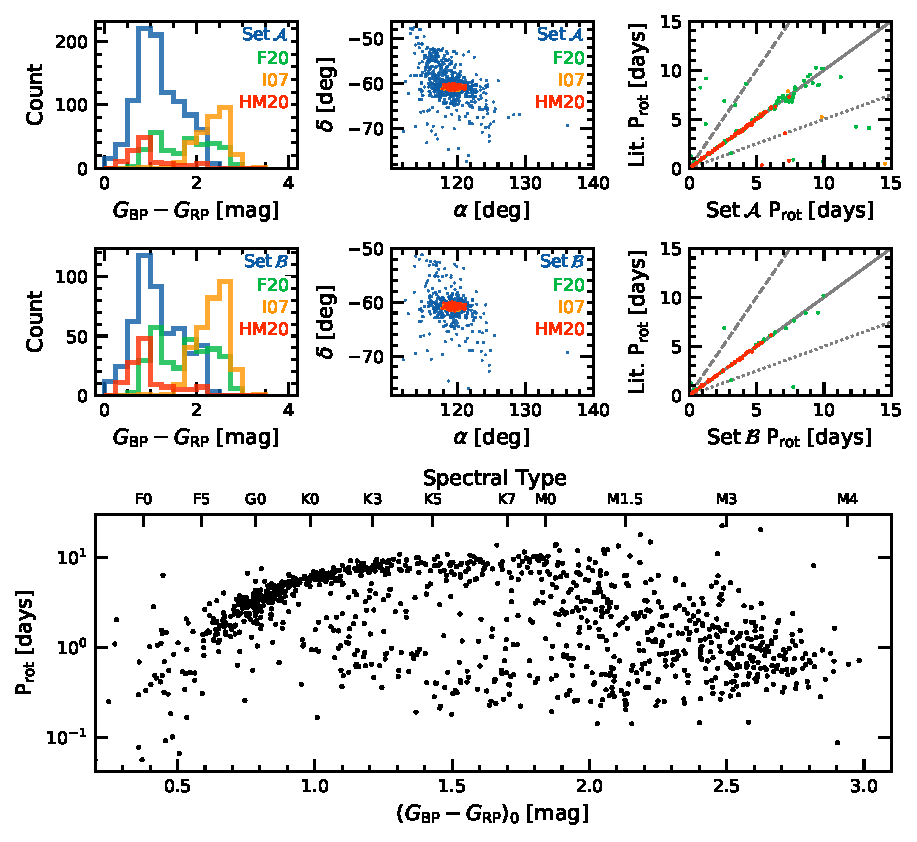
\includegraphics[width=0.3\textwidth]{f10.pdf}
	\end{center}
	\vspace{-0.7cm}
  \caption{ {\bf Different clustering techniques yield different
  candidate members of \cn.} \nkinematic\ unique candidate cluster
  members found using three different techniques are considered in
  this study.  \citetalias{cantatgaudin_gaia_2018}:
  \citet{cantatgaudin_gaia_2018},
  \citetalias{kounkel_untangling_2019}:
  \citet{kounkel_untangling_2019}, \citetalias{meingast_2021}:
  \citet{meingast_2021}.
  \label{fig:venn}
	}
\end{figure}

Figure~\ref{fig:venn} is a Venn diagram of
the three membership catalogs concatenated in this study.  99\% of the
\citetalias{cantatgaudin_gaia_2018} sample overlaps with
\citetalias{kounkel_untangling_2019}, \citetalias{meingast_2021}, or
both.  By comparison, 36\% of the \citetalias{kounkel_untangling_2019}
sample, and 15\% of the \citetalias{meingast_2021} sample do not
overlap with any of the other catalogs.  The data---Gaia DR2---used by
all the studies was the same.  What are the differences in methodology
that produce these different outcomes?

\citetalias{cantatgaudin_gaia_2018} applied a procedure that yielded
what we colloquially call ``the core''.  Their membership assignment
algorithm was to first query a Gaia DR2 cone around the previously
reported $\{\alpha,\delta\}$ of the cluster center, and within $\pm
0.5$\,mas of its previously reported parallax.  The outer radius of
their cone was the previously reported angular radius of the cluster
(0.71$^\circ$; \citealt{Kharchenko_et_al_2013}).  No proper motion cut
was applied.  \citetalias{cantatgaudin_gaia_2018} then applied an
unsupervised classification scheme to $G<18$\,mag stars within this
cone (UPMASK; \citealt{kronemartins_upmask_2014}).  The UPMASK
algorithm first performs a $k$-means clustering on the astrometric
parameters, $\{\mu_{\alpha'}, \mu_\delta, \pi\}$.  A ``veto''
step is then applied to assess whether the groups of stars output from the
$k$-means clustering are more concentrated than a uniform
distribution, by comparing the total branch lengths of their
respective minimum spanning trees.  This binary flag is converted to a
membership probability by redrawing values for $\{\mu_{\alpha'},
\mu_\delta, \pi\}$ using the reported uncertainties and
covariances.  The final membership probability for any given star is
then the fraction of draws for which the star passes the veto step.
In the case of \cn, the resulting radius within which half of the
cluster members were found was 0.50$^\circ$.  We included all
\citetalias{cantatgaudin_gaia_2018} \cn\ members with reported
membership probability exceeding 10\% in our list of candidate cluster
members.

\citetalias{kounkel_untangling_2019} applied a different unsupervised
clustering method to the 5-D Gaia DR2 positions and proper motions.
\citetalias{kounkel_untangling_2019} began with a sample of
$\approx$$2\times 10^7$ stars, mostly within $\approx 1$\,kpc and with
$G\lesssim18$\,mag.  They then applied the hierarchical density-based
spatial clustering of applications with noise algorithm (HDBSCAN;
\citealt{campello_hierarchical_2015}, \citealt{mcinnes_hdbscan_2017})
on the entire sample,  setting the minimum number of stars per cluster
to be 40.  \citetalias{kounkel_untangling_2019} then iterated over a
few different cutoff parallaxes to improve sensitivity to structures
with distances from the Sun ranging between $\approx$100\,pc and
$\approx$1000\,pc.  They then fitted ages to the resulting clusters
using two different methods: isochronal, and a convolutional neural
network.  Regarding membership proabilities,
\citetalias{kounkel_untangling_2019} reported the binary ``member'' or
``not'' from HDBSCAN.
We included all \citetalias{kounkel_untangling_2019} \cn\ members in
our list of candidate cluster members.

Finally, \citetalias{meingast_2021} considered ten known open clusters
within the nearest kiloparsec. One of these clusters was \cn.  Their
initial  list of $\approx$$3\times10^7$ was similar to that of
\citetalias{kounkel_untangling_2019}, mainly requiring well-behaved
astrometry and photometry from Gaia.  Given the mean positions and
velocities of the clusters determined by
\citetalias{cantatgaudin_gaia_2018}, \citetalias{meingast_2021} then
selected all stars with proper-motion correct tangential velocities
within 1.5\,\kms\ of the cluster mean.  They then applied DBSCAN
\citep{ester_density-based_1996} on both the observed galactic
$\{X,Y,Z\}$ coordinates, as well as to a separate deconvolved spatial
coordinate distribution discussed in their Section~3.3.  The results
of their procedure, as well as those of
\citetalias{cantatgaudin_gaia_2018} and
\citetalias{kounkel_untangling_2019}, are visible at the website of
S.~Meingast:
\url{https://homepage.univie.ac.at/stefan.meingast/coronae.html}.
Their reported membership proabilities were binary, similar to those
of \citetalias{kounkel_untangling_2019}.  All of the
\citetalias{meingast_2021} \cn\ members were included in our list of
candidate cluster members.




\section{Considerations for Removing Systematic Variability from TESS Light Curves}
\label{app:detrending}

\begin{figure}[t]
	\begin{center}
		\leavevmode
		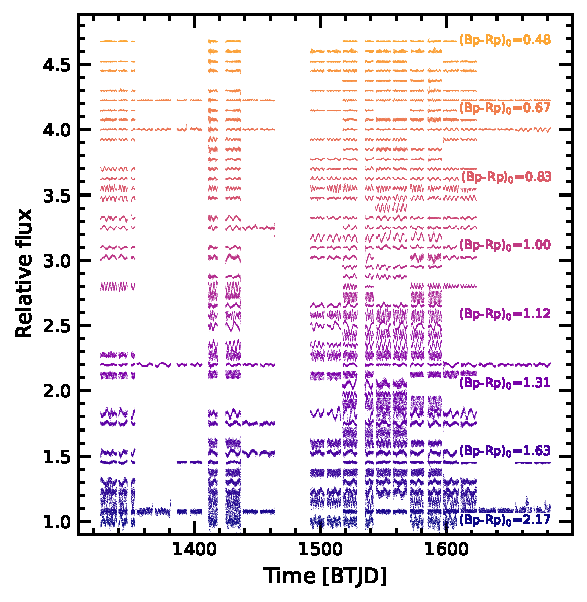
\includegraphics[width=\textwidth]{f14.pdf}
	\end{center}
	\vspace{-1cm}
  \caption{ {\bf \cn\ light curves sorted in order
  of stellar color.} Fifty stars are randomly selected from Set
  $\mathcal{B}$ (see Section~\ref{subsubsec:cluster}), and the light
  curves are detrended and cleaned as discussed in
  Appendix~\ref{app:detrending}.  Each light curve is separated by
  7.5\% in relative flux.  \label{fig:lightcurves}
	}
\end{figure}



In detrending before searching for stellar rotation signals in the
TESS, our goal was to preserve astrophysical variability, while
removing systematic variability.  One particular concern for the TESS
light curves is systematic variability at the timescale of the 14-day
satellite orbit, mostly induced by scattered light from the Earth and
Moon.

We opted to use a variant of the principal component analysis (PCA)
approach discussed by \citet{bouma_cdipsI_2019}. This PCA approach
uses a set of ``trend stars'' selected from across each CCD according
using ad-hoc heuristics that on average lead the trend star light
curves to be dominated by systematic variability.  The resulting
principal component vectors, also referred to as the eigenvectors, are
rank-ordered by the degree of variance that they predict in the
training set of trend stars.

We then posit that any given target star's light curve is described as
a linear combination of the eigenvectors.  We also considered the
inclusion of additional systematic vectors that could affect the light
curve, discussed below.  These can be treated as additional
``features'' in the linear model.  To determine the coefficients of
the linear model after the full set of eigenvectors (plus optional
``sytematic'' vectors) had been asssembled,  we explored two possible
methods: ordinary least squares, and ridge regression. Ridge
regression is the same as ordinary least squares, except it includes
an $\ell^2$ norm with a regularization coefficient. The regularization
coefficient that best applied for any given target light curve was
determined using a cross-validation grid search, through
\texttt{sklearn.linear\_modelRidgeCV} \citep{scikit-learn}.  Each
target light curve was mean-subtracted and normalized by its standard
deviation, as were the eigenvectors. The linear problem was then
solved numerically, and the light curve was reconstructed by re-adding
the original mean, and re-multiplying by the standard deviation to
ensure that the variance of the light curve did not change.

We found that the choice of using ordinary least squares versus ridge
regression did not seem to significantly affect the resulting light
curves. In other words, the inclusion (or lack thereof) of a
regularization term did not strongly alter the best-fitting
coefficients.  In the spirit of keeping it simple, we opted to use
ordinary least squares.  A few other choices seemed to be more
important:

\begin{itemize}
  %
  \item {\it To smooth, or to not smooth the eigenvectors}.
    If the systematic trends are smooth in time, the eigenvectors should be as well. They should not
    contain residuals from {\it e.g.}, eclipsing binaries 
    in the template set, and they should also not be
    intrinsically noisier than the target star. If either of these is
    the case, extra
    variability can be introduced into the ``detrended'' light curves.  To address
    this problem, we opted to smooth the eigenvectors using a
    sliding time-windowed filter (with a "biweight" weight scheme, implemented
    in \texttt{wotan} by \citealt{hippke_wotan_2019}).
    %; window length 1 day, cval 6).
    One issue with this is that systematic sharp features (captured
    e.g., in ``spike vectors'') are no longer captured, so they are present
    in the detrended light curves. Since they can be filtered out in postprocessing
    ({\it e.g.}, using rolling outlier rejection), we prefer this
    approach to having systematic features being injected by the
    PCA detrending.
  %
  \item {\it How many eigenvectors to use}.
    A larger number always leads to greater whitening.  In
    \citet{bouma_cdipsI_2019}, we performed a factor analysis
    cross-validation to determine the number of eigenvectors to use.
    The typical number adopted based on this analysis was 10 to 15.
    While this approach should in theory prevent over-fitting, in our
    experience, for stellar rotation it still often lead to distorts
    the signals, especially for rotation signals with small amplitudes
    and periodicities of $\gtrsim 3$ days.  Shorter signals typically
    are not distorted, since the eigenvectors do not contain the
    high-frequency content that leads to the distortions.  For the
    present analysis, we therefore set the maximum number of
    eigenvectors to be 5.
%
  \item {\it Which supplementary systematics vectors to use}.  We
    considered using the \texttt{BGV}, \texttt{CCDTEMP}, \texttt{XIC},
    \texttt{YIC}, and \texttt{BGV} vectors, packaged with the CDIPS
    light curves. We found that the background value measured in an
    annulus centered on the aperture, \texttt{BGV}, tended to produce
    the best independent information from the PCA eigenvectors, and so
    we adopted it as our only ``supplementary'' trend vector.  We
    opted to not smooth it, assuming that it would provide direct
    complement to the smoothed PCA vectors.
\end{itemize}

After all these considerations, for every ``target star'', we
ultimately decorrelated the raw (image-subtracted and
background-subtracted) light curve using a linear model with ordinary
least squares.  The vectors used in the model were the 1
unsmoothed background flux vector, and 5 smoothed PCA eigenvectors.
Figure~\ref{fig:lightcurves} shows fifty light curves
randomly drawn from the resulting ``Set $\mathcal{B}$''.




\section{Comparison Star Rotation Periods}
\label{app:compstar}

\begin{figure}[t]
	\begin{center}
		\leavevmode
    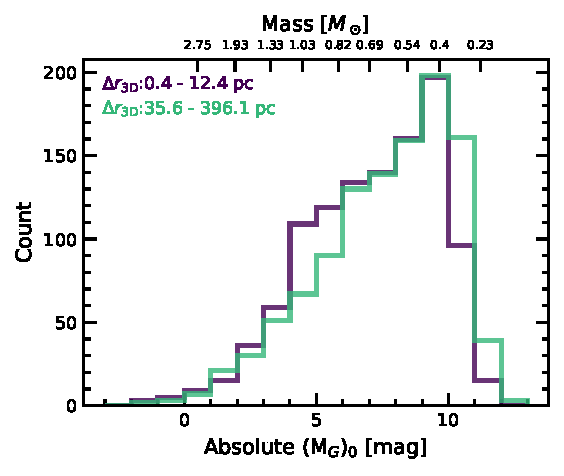
\includegraphics[width=0.49\textwidth]{f9.pdf}
	\end{center}
	\vspace{-0.7cm}
	\caption{ {\bf Rotation in NGC\,2516 compared to the field.}
  Stars with Gaia $Rp<13$\,mag in the cluster and field samples were
  considered. (Fainter stars in the field sample were not studied as
  part of the broader CDIPS project).  The field stars show a
  different rotation period distribution than the kinematically
  selected NGC\,2516 members.
  {\bf LGB TODO: Rerun the field measurements with a better grid to fix the aliasing issue.}
  \label{fig:compstar}
	}
\end{figure}

To provide a basis for comparison, we also opted to search the
``calibration'' light curves ($Rp<13$) that were created as a part of
the CDIPS project.  Over the southern sky (Sectors 1-13 of TESS), this
corresponded to a sample of \ncalibration\ stars.  Cross-matching these
against the \nnbhd\ randomly drawn stars in the neighborhood of \cn yielded
\nnbhdcalibstar\ unique stars, with a cumulative total of
\nnbhdcaliblc\ TESS
sectors observed.
The magnitude cut of $Rp<13$ at the distances of the neighborhood sample
corresponds to an extinction-corrected color cutoff of $\bpmrp
\approx 0.80$, or spectral types of $\approx$G1V.
This reaches sufficiently far down the main-sequence to enable a
comparison to the cluster star sample.

We performed the same light curve stitching and period-search
procedure on the field comparison stars.
Imposing the same requirements for crowding resulted in
\ncompstardenominator\ stars for which rotation periods could have been
detected.
Imposing the same Lomb Scargle power cutoff, and period upper limit,
yielded \ncompstarnumerator\ period detections (\ncompfrac).
Within the same brightness cutoff, 
\nautovscompstarnumerator\ of \nautovscompstardenominator\ cluster stars
yielded period detections (\nautofrac).
Though the detection fractions are frankly not very different
(likely because of the brightness cutoff), the period {\it
vs} color distributions are quite different
(Figure~\ref{fig:compstar}).


\section{Projection effects for 2D velocities}
\label{app:vproj}

\begin{figure}[t]
	\begin{center}
		\leavevmode
		\subfloat{
			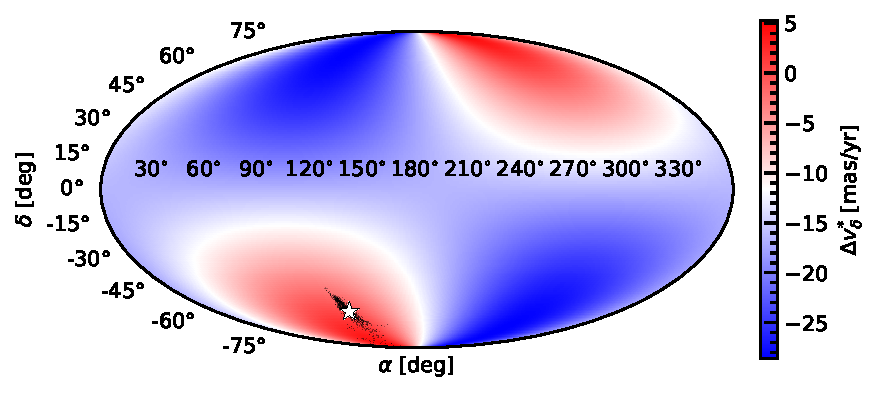
\includegraphics[width=0.49\textwidth]{f12a.pdf}
		}

		\subfloat{
			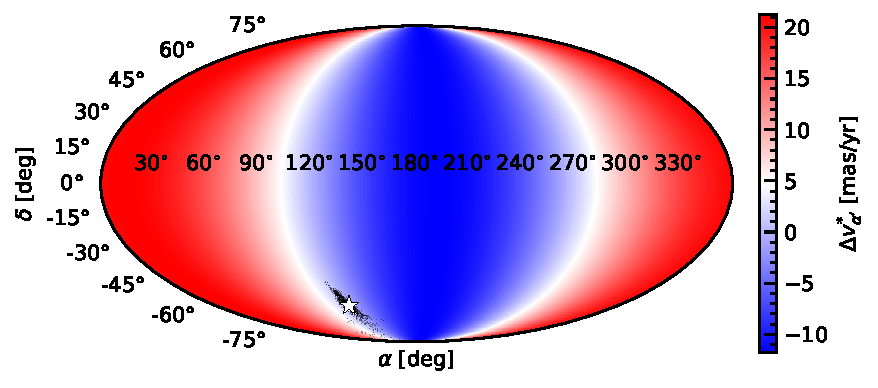
\includegraphics[width=0.49\textwidth]{f12b.pdf}
		}
	\end{center}
	\vspace{-0.7cm}
  \caption{ {\bf Projection effects for co-moving populations across
  the sky.} The map is colored by the velocity difference a star
  co-moving with \cn\ would exhibit across the equatorial sphere.
  Actual positions of candidate \cn\ members are shown with points;
  the star denotes the cluster center.
	\label{fig:vproj}
	}
\end{figure}

Figure~\ref{fig:vproj} shows why the correct approach for comparing
any star's proper motions against the cluster's mean depends on the
position of the star being considered.


% \section{Differential Reddening}
% \label{app:diffred}
% 
% \begin{figure*}[t]
% 	\begin{center}
% 		\leavevmode
% 			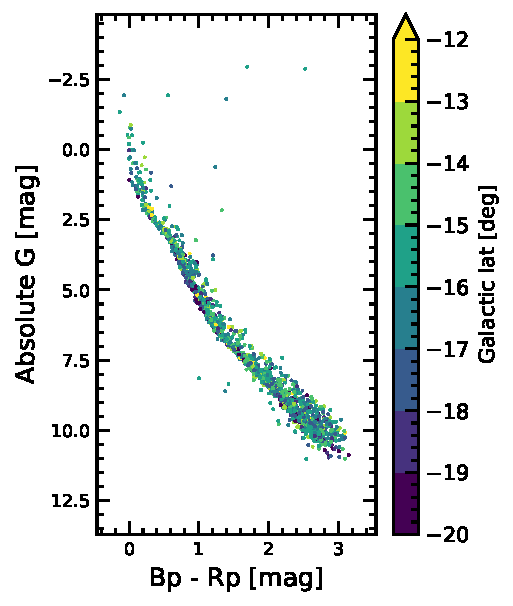
\includegraphics[width=0.75\textwidth]{f2c.pdf}
% 	\end{center}
% 	\vspace{-0.7cm}
%   \caption{ {\bf HR diagram of NGC\,2516, using Gaia EDR3 photometry.}
%     {\it Bottom:} Reported members of the halo, as a function of
%     galactic latitude. Can the additional scatter in the halo be
%     understood through differential reddening?
%     {\bf Maybe}.
%     \label{fig:diffred}
%   }
% \end{figure*}
% 
% Figure~\ref{fig:diffred}.


% \section{Kinematics $\otimes$ Rotation}
% \label{app:gaia6d_x_rotn}
% 
% \begin{figure*}[t]
% 	\begin{center}
% 		\leavevmode
% 		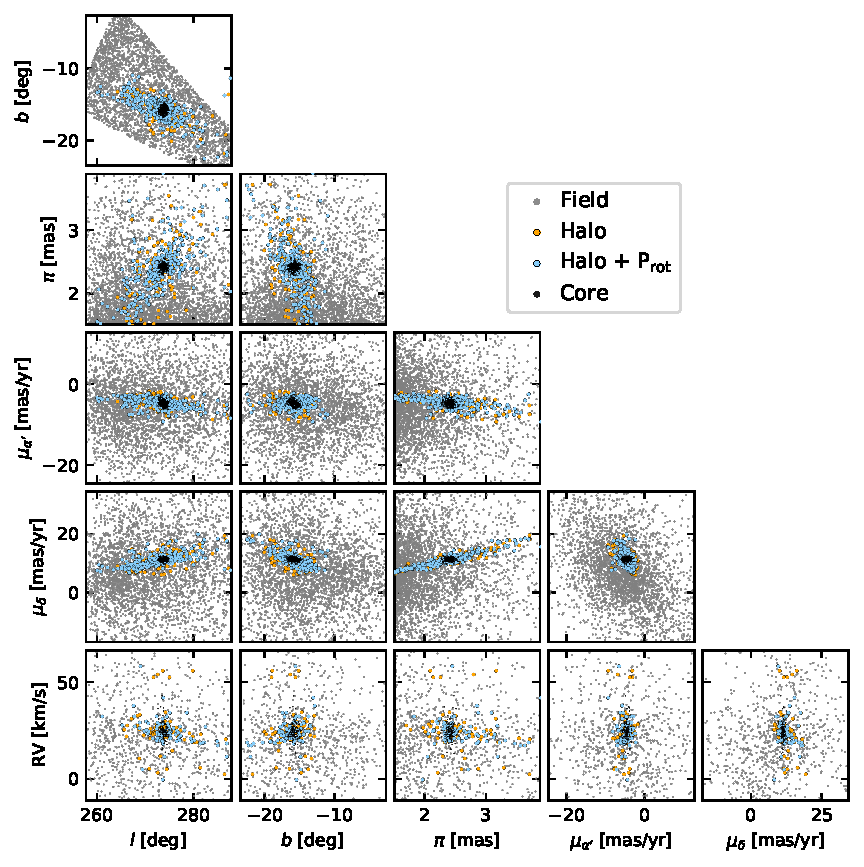
\includegraphics[width=0.95\textwidth]{f4.pdf}
% 	\end{center}
% 	\vspace{-0.7cm}
%   \caption{ {\bf Gaia-based components of NGC\,2516 in position and
%   velocity space, cross-matched against the rotators.} The plotted
%   stars are those with $0.5<\bpmrp<1.2$ that meet the crowding
%   restrictions described in Section~\ref{subsec:tess}: they should
%   have been sufficiently bright and non-crowded to enable rotation
%   period detection.  We caution that the appearance of fewer
%   non-rotators being present toward the core is due the layering of
%   the plot: quantitatively, stars toward the cluster center do not all
%   show rotation periods in our analysis (see
%   Figure~\ref{fig:hist_physical_x_rotn}).
%   \label{fig:gaia6d_x_rotn}
% 	}
% \end{figure*}
% 
% Figure~\ref{fig:gaia6d_x_rotn} is an alternative visualization of the
% data shown in Figure~\ref{fig:physical_x_rotn}.  The rotation periods
% in this diagram correspond to ``Set $\mathcal{A}$'' as described in
% Section~\ref{subsec:tess}.  Many stars in the outer region of the
% cluster show rotation periods consistent with a young age.  One issue
% with the visualization as displayed however is that it hides the
% amount of non-rotators toward the cluster center: we did not detect
% rotation periods for roughly one in four stars at the cluster
% center (see Figures~\ref{fig:physical_x_rotn}
% and~\ref{fig:hist_physical_x_rotn}).
% 
% 
% 
% \section{Rotation $\otimes$ RUWE}
% \label{app:ruwe}
% 
% \begin{figure*}[t]
% 	\begin{center}
% 		\leavevmode
% 		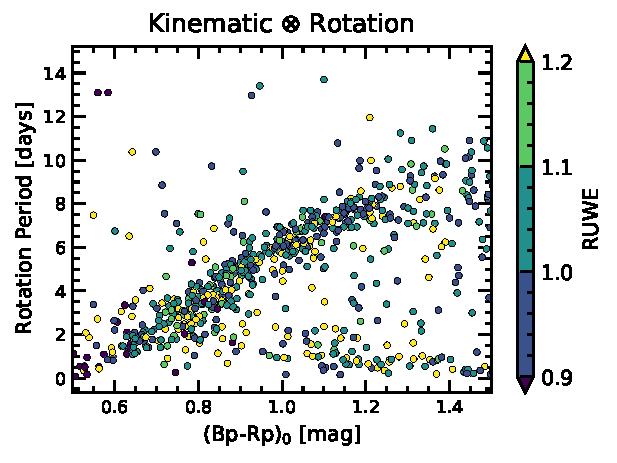
\includegraphics[width=0.95\textwidth]{f6.pdf}
% 	\end{center}
% 	\vspace{-0.7cm}
% 	\caption{ {\bf Rotation versus color, colored by RUWE.}
% 		Looks like on the slow sequence, there's more yellow at the bottom?
% 		\label{fig:rotn_X_RUWE}
% 	}
% \end{figure*}
% 
% Figure~\ref{fig:rotn_X_RUWE}.
% 
% 
% \section{Kinematics $\otimes$ Rotation in EDR3}
% 
% \begin{figure*}[t]
% 	\begin{center}
% 		\leavevmode
% 		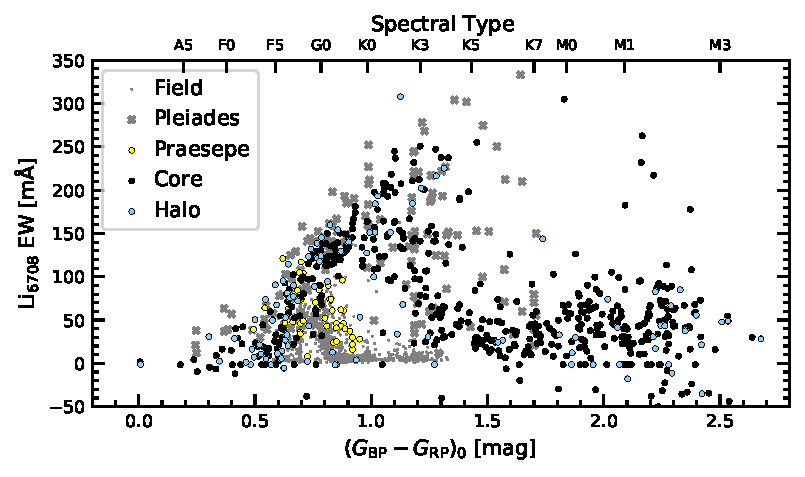
\includegraphics[width=0.95\textwidth]{f7.pdf}
% 	\end{center}
% 	\vspace{-0.7cm}
% 	\caption{ {\bf Gaia-based components of NGC\,2516 in position and
%     velocity space, cross-matched against the rotators. Analog of
%     Figure~\ref{fig:gaia6d_x_rotn}, but showing EDR3 kinematics.}
% 		\label{fig:gaia6d_x_rotn_EDR3}
% 	}
% \end{figure*}
% 
% How did we do?
% Figure~\ref{fig:gaia6d_x_rotn_EDR3} lets us check with a more precise
% astrometric solution.






\listofchanges

%\allauthors
\end{document}
